% Options for packages loaded elsewhere
\PassOptionsToPackage{unicode}{hyperref}
\PassOptionsToPackage{hyphens}{url}
%
\documentclass[
  man,mask,floatsintext]{apa7}
\usepackage{amsmath,amssymb}
\usepackage{iftex}
\ifPDFTeX
  \usepackage[T1]{fontenc}
  \usepackage[utf8]{inputenc}
  \usepackage{textcomp} % provide euro and other symbols
\else % if luatex or xetex
  \usepackage{unicode-math} % this also loads fontspec
  \defaultfontfeatures{Scale=MatchLowercase}
  \defaultfontfeatures[\rmfamily]{Ligatures=TeX,Scale=1}
\fi
\usepackage{lmodern}
\ifPDFTeX\else
  % xetex/luatex font selection
\fi
% Use upquote if available, for straight quotes in verbatim environments
\IfFileExists{upquote.sty}{\usepackage{upquote}}{}
\IfFileExists{microtype.sty}{% use microtype if available
  \usepackage[]{microtype}
  \UseMicrotypeSet[protrusion]{basicmath} % disable protrusion for tt fonts
}{}
\makeatletter
\@ifundefined{KOMAClassName}{% if non-KOMA class
  \IfFileExists{parskip.sty}{%
    \usepackage{parskip}
  }{% else
    \setlength{\parindent}{0pt}
    \setlength{\parskip}{6pt plus 2pt minus 1pt}}
}{% if KOMA class
  \KOMAoptions{parskip=half}}
\makeatother
\usepackage{xcolor}
\usepackage{graphicx}
\makeatletter
\def\maxwidth{\ifdim\Gin@nat@width>\linewidth\linewidth\else\Gin@nat@width\fi}
\def\maxheight{\ifdim\Gin@nat@height>\textheight\textheight\else\Gin@nat@height\fi}
\makeatother
% Scale images if necessary, so that they will not overflow the page
% margins by default, and it is still possible to overwrite the defaults
% using explicit options in \includegraphics[width, height, ...]{}
\setkeys{Gin}{width=\maxwidth,height=\maxheight,keepaspectratio}
% Set default figure placement to htbp
\makeatletter
\def\fps@figure{htbp}
\makeatother
\setlength{\emergencystretch}{3em} % prevent overfull lines
\providecommand{\tightlist}{%
  \setlength{\itemsep}{0pt}\setlength{\parskip}{0pt}}
\setcounter{secnumdepth}{-\maxdimen} % remove section numbering
% Make \paragraph and \subparagraph free-standing
\ifx\paragraph\undefined\else
  \let\oldparagraph\paragraph
  \renewcommand{\paragraph}[1]{\oldparagraph{#1}\mbox{}}
\fi
\ifx\subparagraph\undefined\else
  \let\oldsubparagraph\subparagraph
  \renewcommand{\subparagraph}[1]{\oldsubparagraph{#1}\mbox{}}
\fi
\newlength{\cslhangindent}
\setlength{\cslhangindent}{1.5em}
\newlength{\csllabelwidth}
\setlength{\csllabelwidth}{3em}
\newlength{\cslentryspacingunit} % times entry-spacing
\setlength{\cslentryspacingunit}{\parskip}
\newenvironment{CSLReferences}[2] % #1 hanging-ident, #2 entry spacing
 {% don't indent paragraphs
  \setlength{\parindent}{0pt}
  % turn on hanging indent if param 1 is 1
  \ifodd #1
  \let\oldpar\par
  \def\par{\hangindent=\cslhangindent\oldpar}
  \fi
  % set entry spacing
  \setlength{\parskip}{#2\cslentryspacingunit}
 }%
 {}
\usepackage{calc}
\newcommand{\CSLBlock}[1]{#1\hfill\break}
\newcommand{\CSLLeftMargin}[1]{\parbox[t]{\csllabelwidth}{#1}}
\newcommand{\CSLRightInline}[1]{\parbox[t]{\linewidth - \csllabelwidth}{#1}\break}
\newcommand{\CSLIndent}[1]{\hspace{\cslhangindent}#1}
\ifLuaTeX
\usepackage[bidi=basic]{babel}
\else
\usepackage[bidi=default]{babel}
\fi
\babelprovide[main,import]{english}
% get rid of language-specific shorthands (see #6817):
\let\LanguageShortHands\languageshorthands
\def\languageshorthands#1{}
% Manuscript styling
\usepackage{upgreek}
\captionsetup{font=singlespacing,justification=justified}

% Table formatting
\usepackage{longtable}
\usepackage{lscape}
% \usepackage[counterclockwise]{rotating}   % Landscape page setup for large tables
\usepackage{multirow}		% Table styling
\usepackage{tabularx}		% Control Column width
\usepackage[flushleft]{threeparttable}	% Allows for three part tables with a specified notes section
\usepackage{threeparttablex}            % Lets threeparttable work with longtable

% Create new environments so endfloat can handle them
% \newenvironment{ltable}
%   {\begin{landscape}\centering\begin{threeparttable}}
%   {\end{threeparttable}\end{landscape}}
\newenvironment{lltable}{\begin{landscape}\centering\begin{ThreePartTable}}{\end{ThreePartTable}\end{landscape}}

% Enables adjusting longtable caption width to table width
% Solution found at http://golatex.de/longtable-mit-caption-so-breit-wie-die-tabelle-t15767.html
\makeatletter
\newcommand\LastLTentrywidth{1em}
\newlength\longtablewidth
\setlength{\longtablewidth}{1in}
\newcommand{\getlongtablewidth}{\begingroup \ifcsname LT@\roman{LT@tables}\endcsname \global\longtablewidth=0pt \renewcommand{\LT@entry}[2]{\global\advance\longtablewidth by ##2\relax\gdef\LastLTentrywidth{##2}}\@nameuse{LT@\roman{LT@tables}} \fi \endgroup}

% \setlength{\parindent}{0.5in}
% \setlength{\parskip}{0pt plus 0pt minus 0pt}

% Overwrite redefinition of paragraph and subparagraph by the default LaTeX template
% See https://github.com/crsh/papaja/issues/292
\makeatletter
\renewcommand{\paragraph}{\@startsection{paragraph}{4}{\parindent}%
  {0\baselineskip \@plus 0.2ex \@minus 0.2ex}%
  {-1em}%
  {\normalfont\normalsize\bfseries\itshape\typesectitle}}

\renewcommand{\subparagraph}[1]{\@startsection{subparagraph}{5}{1em}%
  {0\baselineskip \@plus 0.2ex \@minus 0.2ex}%
  {-\z@\relax}%
  {\normalfont\normalsize\itshape\hspace{\parindent}{#1}\textit{\addperi}}{\relax}}
\makeatother

% \usepackage{etoolbox}
\makeatletter
\patchcmd{\HyOrg@maketitle}
  {\section{\normalfont\normalsize\abstractname}}
  {\section*{\normalfont\normalsize\abstractname}}
  {}{\typeout{Failed to patch abstract.}}
\patchcmd{\HyOrg@maketitle}
  {\section{\protect\normalfont{\@title}}}
  {\section*{\protect\normalfont{\@title}}}
  {}{\typeout{Failed to patch title.}}
\makeatother

\usepackage{xpatch}
\makeatletter
\xapptocmd\appendix
  {\xapptocmd\section
    {\addcontentsline{toc}{section}{\appendixname\ifoneappendix\else~\theappendix\fi\\: #1}}
    {}{\InnerPatchFailed}%
  }
{}{\PatchFailed}
\keywords{social-cognitive development, theory of mind, gaze cues, individual differences, cognitive modeling, lifespan\newline\indent Word count: 7914}
\usepackage{lineno}

\linenumbers
\usepackage{csquotes}
\usepackage{setspace}
\captionsetup[figure]{font={stretch=1}}
\makeatletter
\renewcommand{\paragraph}{\@startsection{paragraph}{4}{\parindent}%
  {0\baselineskip \@plus 0.2ex \@minus 0.2ex}%
  {-1em}%
  {\normalfont\normalsize\bfseries\typesectitle}}

\renewcommand{\subparagraph}[1]{\@startsection{subparagraph}{5}{1em}%
  {0\baselineskip \@plus 0.2ex \@minus 0.2ex}%
  {-\z@\relax}%
  {\normalfont\normalsize\bfseries\itshape\hspace{\parindent}{#1}\textit{\addperi}}{\relax}}
\makeatother

\ifLuaTeX
  \usepackage{selnolig}  % disable illegal ligatures
\fi
\IfFileExists{bookmark.sty}{\usepackage{bookmark}}{\usepackage{hyperref}}
\IfFileExists{xurl.sty}{\usepackage{xurl}}{} % add URL line breaks if available
\urlstyle{same}
\hypersetup{
  pdftitle={Variation in gaze understanding across the life span: A process-level perspective},
  pdflang={en-EN},
  pdfkeywords={social-cognitive development, theory of mind, gaze cues, individual differences, cognitive modeling, lifespan},
  hidelinks,
  pdfcreator={LaTeX via pandoc}}

\title{Variation in gaze understanding across the life span: A process-level perspective}
\author{Julia Christin Prein\textsuperscript{1}, Luke Maurits\textsuperscript{1}, Annika Werwach\textsuperscript{3,4}, Daniel B. M. Haun\textsuperscript{1,*}, \& Manuel Bohn\textsuperscript{1,2,*}}
\date{}


\shorttitle{modeling variation in gaze understanding}

\authornote{

The authors made the following contributions. Julia Christin Prein: Conceptualization, Methodology, Software, Investigation, Formal Analysis, Writing - Original Draft Preparation, Writing - Review \& Editing; Luke Maurits: Formal Analysis, Writing - Review \& Editing; Annika Werwach: Methodology, Investigation, Writing - Review \& Editing; Daniel B. M. Haun: Supervision, Writing - Review \& Editing; Manuel Bohn: Conceptualization, Formal Analysis, Writing - Original Draft Preparation, Writing - Review \& Editing.

Correspondence concerning this article should be addressed to Julia Christin Prein, Max Planck Institute for Evolutionary Anthropology, Deutscher Platz 6, 04103 Leipzig, Germany. E-mail: \href{mailto:julia_prein@eva.mpg.de}{\nolinkurl{julia\_prein@eva.mpg.de}}

}

\affiliation{\vspace{0.5cm}\textsuperscript{1} Department of Comparative Cultural Psychology, Max Planck Institute for Evolutionary Anthropology, Leipzig, Germany\\\textsuperscript{2} Institute of Psychology, Leuphana University Lüneburg, Germany\\\textsuperscript{3} Center for Lifespan Psychology, Max Planck Institute for Human Development, Berlin, Germany\\\textsuperscript{4} Max Planck School of Cognition, Leipzig, Germany\\\textsuperscript{*} Shared senior authorship}

\abstract{%
Following eye gaze is fundamental for many social-cognitive abilities, for example, when judging what another agent can or cannot know. While the emergence of gaze-following has been thoroughly studied on a group level, we know little about (a) the developmental trajectory beyond infancy and (b) the sources of individual differences. In Study 1, we examined gaze understanding across the lifespan (\emph{N} = 471 3- to 80-years-olds; children from a mid-sized German city; international remotely tested adults). We found a steep performance improvement during preschool years, in which children became more precise in locating the attentional focus of an agent. Precision levels then stayed comparably stable throughout adulthood with a minor decline toward old age. In Study 2, we formalized the process of gaze understanding in a computational cognitive model that allowed us to conceptualize individual differences in a psychologically meaningful way (\emph{N} = 60 3- to 5-year-olds, 50 adults). According to our model, participants estimate pupil angles with varying levels of precision based on observing the pupil location within the agent's eyes. In Study 3, we tested two implications of our gaze model, namely that gaze understanding could be related to vector estimation in non-social settings and perspective-taking abilities (\emph{N} = 102 4- to 5-year-olds). We found that gaze understanding is associated with both of these abilities but less so with other Theory of Mind tasks. This work illustrates how the combination of reliable measurement instruments and formal theoretical models allows us to explore the in(ter)dependence of core social-cognitive processes in greater detail.
}



\begin{document}
\maketitle

\hypertarget{variation-in-gaze-understanding-across-the-life-span-a-process-level-perspective}{%
\section{Variation in gaze understanding across the life span: A process-level perspective}\label{variation-in-gaze-understanding-across-the-life-span-a-process-level-perspective}}

\textbf{Authors:} Julia Christin Prein\textsuperscript{1}, Luke Maurits\textsuperscript{1}, Annika Werwach\textsuperscript{1,3,4}, Daniel B. M. Haun\textsuperscript{1,*}, Manuel Bohn\textsuperscript{1,2,*}

\textbf{Affiliations:} \textsuperscript{1} Department of Comparative Cultural Psychology, Max Planck Institute for Evolutionary Anthropology, Leipzig, Germany.
\textsuperscript{2} Institute of Psychology, Leuphana University Lüneburg, Germany.
\textsuperscript{3} Center for Lifespan Psychology, Max Planck Institute for Human Development, Berlin, Germany.
\textsuperscript{4} Max Planck School of Cognition, Leipzig, Germany.
\textsuperscript{*} shared senior authorship

\textbf{ORCiD}: \emph{Julia Christin Prein} \url{https://orcid.org/0000-0002-3154-6167}

\textbf{Conflicts of interest:} The authors declare that they have no conflict of interest.

\textbf{Data availability statement:} The web application (\url{https://ccp-odc.eva.mpg.de/tango-demo/}) described here is open source (\url{https://github.com/ccp-eva/tango-demo}). The data sets generated during and/or analyzed during the current study are available in the {[}gazecues-modeling{]} repository (\url{https://github.com/ccp-eva/gazecues-modeling}). All experiments were pre-registered (\url{https://osf.io/zjhsc/}).

\textbf{Acknowledgements:} We thank Jana Jurkat for her help with data collection and participant recruitment. We would also like to thank Steven Kalinke for his technical programming support. We thank all the children, caregivers, and adults who participated in the study.

\textbf{Funding:} This study was funded by the Max Planck Society for the Advancement of Science, a noncommercial, publicly financed scientific organization (no grant number). Manuel Bohn was supported by a Jacobs Foundation Research Fellowship.

\textbf{Ethical statement:} The study obtained ethical clearance by the MPG Ethics commission Munich, Germany, falling under an umbrella ethics application (Appl. No.~2021\_45). Informed consent was obtained from all individual participants or their legal guardians. The research adhered to the legal requirements of psychological research with children in Germany.

\newpage

\hypertarget{research-highlights-to-be-placed-before-the-abstract}{%
\section{Research highlights (to be placed before the abstract)}\label{research-highlights-to-be-placed-before-the-abstract}}

\begin{itemize}
\tightlist
\item
  Gaze understanding develops beyond infancy. Highest precision levels in localizing attentional foci are reached in young adulthood with a slight decrease towards old age.
\item
  We present a computational model as a mechanistic description of gaze understanding. The model explains individual differences and recovers signature patterns in the data.
\item
  Our model assumes that gaze understanding relies on vector estimation. To test this assumption experimentally, we designed a non-social vector estimation task.
\item
  We found substantial correlations between gaze understanding and vector estimation, as well as Level 2 perspective-taking. Other Theory of Mind tasks did not correlate.
\end{itemize}

\hypertarget{introduction}{%
\section{Introduction}\label{introduction}}

Following the gaze of others is valuable to extract information from the environment. It guides us to ``informational hotspots'' (Meltzoff et al., 2010, p. 1) and can be used to identify internal states such as intentions or emotions (Corkum \& Moore, 1998; Pfeiffer et al., 2013). As one of the most fundamental social-cognitive abilities, gaze-following is an integral part of almost every form of social interaction, including communication, collaboration, cultural and social learning (Bohn \& Frank, 2019; Emery, 2000; Frith \& Frith, 2012; Hessels, 2020; Moore, 2008; Rakoczy, 2022; Tomasello \& Rakoczy, 2003), and has been extensively studied in infancy (for review, see Del Bianco et al., 2019). In the most commonly used paradigm (e.g., Astor et al., 2020; Byers-Heinlein et al., 2021; Gredebäck et al., 2010; Ishikawa et al., 2022), the experimenter looks directly at the infant before shifting their head and eyes to one of the two objects. Infants' looking times to the target or the proportion of choosing the target over the distractor are measured. Analyses traditionally focus on the average age at which children as a group reach an above-chance performance. Research in this tradition finds that infants as young as six months can follow gaze to that of another agent (D'Entremont et al., 1997). At the end of their first year of life, infants can follow gaze to locations outside their current visual field and move themselves to gain proper perceptual access (Butterworth \& Jarrett, 1991; Corkum \& Moore, 1995; Deák et al., 2000; Moll \& Tomasello, 2004).

While the emergence of gaze-following has been well established, less is known about its developmental trajectory beyond infancy. One possibility is that the ability to follow gaze does not improve once it emerges. Yet, most, if not all, cognitive abilities continue to develop throughout childhood (e.g., Gathercole et al., 2004; Gredebäck et al., 2010). It seems likely that children fine-tune their gaze understanding as they get older - presumably while using them in social interactions. To capture development in gaze understanding beyond infancy, we conducted our Study 1 across the lifespan.

Up until today, only a handful of gaze-following studies differentiate between manipulating head and eye movement. Michel et al. (2021) found that gaze-following in four-month-olds was likely driven by other's head- instead of eye movements. Corkum and Moore (1995), Lempers (1979), and Lempers et al. (1977) suggest that infants, at least until 19 months, struggle when eye and head direction diverge. From farther distance, body or face orientation can act as more salient cues to determine another's area of attention. However, eye direction indicates a more precise location of focus (Emery, 2000), and allows to anticipate likely future actions (Friesen \& Rao, 2011; Zohary et al., 2022). In our three studies, we therefore focused on subtle gaze cues and isolated eye movement alone.

Though previous studies suggest that young infants can align their visual attention to another's line of sight, this does not necessarily indicate understanding the intentions of the agent (Aslin, 2007). Infants could simply align their orientation without processing what exactly the other is seeing (Butterworth \& Jarrett, 1991). In fact, one might question if such an alignment reflects an understanding of visual perspectives at all, because the ``target'' or ``object of representation'' is not necessarily specified (Perner et al., 2003, p. 358). To fulfill this criterion, Moll and Tomasello (2006) applied an active behavioral choice, in which participants searched for a visually accessible or inaccessible target object. 24-month-olds succeeded in the task, while 18-month-olds did not. In an object choice study with two containers, Behne et al. (2005) found that already 14-month-olds used an experimenter's gaze; however, this was again confounded with a congruent face movement (cf. Povinelli et al., 1997). In our three studies, we assessed how subtle gaze cues guided participants' behavior in actively locating a target.

Finally, group-level analyses of gaze-following abilities may mask individual differences between children. Measuring individual differences in basic aspects of social cognition is especially important to understand the underlying processes and to quantify the impact of environmental influences and other cognitive abilities (Birch et al., 2017; Del Bianco et al., 2019). In our studies, we measured gaze understanding continuously by using a task which is designed to capture individual-level variation (Prein et al., 2023).

The present study had two main goals: first, we studied the development of gaze understanding beyond infancy (Study 1). Instead of capturing the youngest age at which children follow gaze, we examined how this ability changes with age. Our second goal was to provide a process-level theory of gaze understanding (and individual differences therein) as a computational cognitive model. We formalized gaze understanding as a form of vector estimation and tested whether our model explained empirical data (Study 2). Finally, we examined two empirical predictions that followed from the model, namely that gaze understanding is related to non-social vector estimation and visual perspective-taking (Study 3).

\hypertarget{study-1-gaze-understanding-across-the-lifespan}{%
\section{Study 1: Gaze understanding across the lifespan}\label{study-1-gaze-understanding-across-the-lifespan}}

The study was pre-registered at: \url{https://osf.io/snju6} (child sample) and \url{https://osf.io/6yjz3} (adult sample). The study obtained ethical clearance by the MPG Ethics commission Munich, Germany, falling under an umbrella ethics application (Appl. No.~2021\_45). Data was collected between May 2021 and April 2023.

\hypertarget{participants}{%
\subsection{Participants}\label{participants}}

We collected data online from 3- to 80- year-olds (see Supplements for further details). The child sample consisted of 471 participants and was recruited via an internal database of families in Leipzig, Germany, who volunteered to participate in child development studies. Participants came from ethnically homogeneous, mixed socioeconomic backgrounds with mid to high parental education levels. They lived in an industrialized, urban Central-European context in a mid-size German city (approx. 600,000 inhabitants; median individual monthly net income approx. 1,600€ as of 2021). Most were raised monolingually in a nuclear two-generational family setting. Information on demographics and socioeconomic status was not formally recorded on a participant level.

Adults were recruited via \emph{Prolific} (Palan \& Schitter, 2018). \emph{Prolific} is an online participant recruitment tool from the University of Oxford with predominantly European and US-American subjects. Participants consisted of 240 English-speaking adults who reported to have normal or corrected-to-normal vision. For completing the study, subjects were paid above the fixed minimum wage (\textasciitilde£10.00/hour).

\hypertarget{materials}{%
\subsection{Materials}\label{materials}}

We used the continuous version of the TANGO (Prein et al., 2023). The task was presented as a web application (demo \href{https://ccp-odc.eva.mpg.de/tango-demo/.}{https://ccp-odc.eva.mpg.de/tango-demo/}; source code \url{https://github.com/ccp-eva/tango-demo}). The TANGO showed satisfactory internal consistency and retest reliability for children and adults (reliability estimates \emph{Pearson's r} from .7 to .8; (Prein et al., 2023)).

\hypertarget{procedure}{%
\subsection{Procedure}\label{procedure}}

Children and teenagers received a personalized link to the study website. Caregivers were asked to provide technical support, while explicitly being reminded not to help in responding. Webcam videos were recorded whenever consented and technically feasible in order to monitor whether children and teenagers responded on their own. Adults completed the online study unsupervised.

Each trial presented an agent standing in a window, watching a balloon (\emph{i.e.}, target) falling to the ground (see Figure \ref{fig:fig4}A; however, Study 1 presented animal agents). The target fell behind a hedge while the agent's gaze followed the target's trajectory. In test trials, a hedge covered the target's position. Participants were asked to touch or click where they estimated the target to be based on the agent's gaze. Four familiarization trials ensured participants understood the task and felt comfortable with the response format. Then, 15 test trials followed. Completing 19 trials took 5-10 minutes.

We measured imprecision, defined as the absolute difference between the target center and the x coordinate of the participant's click. The screen width was divided into ten bins. Within each bin, exact target coordinates were randomly generated. Each target bin, agent, and target color occurred equally often and did not appear in more than two consecutive trials.

\hypertarget{analysis}{%
\subsection{Analysis}\label{analysis}}

We ran all analyses in R version 4.3.2 (2023-10-31) (R Core Team, 2022). Regression models were fit as Bayesian generalized linear mixed models (GLMMs) with default priors using the function \texttt{brm} from the package \texttt{brms} (Bürkner, 2017, 2018).

We fit GLMMs that make different assumptions about the developmental trajectory, modeling the relationship between age and performance as linear, quadratic, or cubic. In addition, we fit a Gaussian Process model (Bürkner, 2017), which assumes a smooth relationship but avoids enforcing a particular shape. Per individuum, imprecision was aggregated across trials and modeled as a \texttt{lognormal} distribution.\footnote{Originally, we fit our models on a trial-by-trial basis with the following structure: \texttt{performance\ \textasciitilde{}\ age\ +\ symmetricPosition\ +\ trialNr\ +\ (1\ +\ symmetricPosition\ +\ trialNr\ \textbar{}\ subjID)}. However, the Gaussian Process model was computationally heavy. Thus, we simplified the model structure, aggregated data on a subject level, and included only age as an effect. See Supplements for a comparison between the original and the here-reported model structures. The model predictions did not differ notably.} The unit of imprecision was counted in target widths, i.e., an imprecision of 1 meant clicking one balloon width to the left or right of the true target center. We inspected the posterior distributions (mean and 95\% Credible Interval (CrI)) for the age estimates and compared models via model weights and the difference in expected log pointwise predictive density (ELPD) estimated using leave-one-out cross-validation (LOO) (Vehtari et al., 2017).

To obtain a concise but principled characterization of the developmental trajectory, we additionally performed a Bayesian change point analysis, using the package \texttt{RBeast} (Zhao et al., 2019). We sought the most likely change points in our data, assuming a constant mean (i.e., a flat line, zero degree polynomial) within each segment. To avoid ``overreactions'' to outlying data points, we constrained the model to have minimally 10 data points between consecutive change points (= half of the data points collected per adult decade). We inspected the posterior probability of different numbers of change points and the locations of these change points (mean and 95\% CrI).\footnote{In a supplementary analysis, we varied the parameters of our change point analysis and modified the number of allowed change points, the minimum number of data points between change points, and the polynomial order. When we allowed more explorative room, the models became more sensitive and added more fine-grained change points. The exact location of the change points varied slightly. However, the overall interpretation stayed the same, fitting our initial visual inspection: while early childhood was characterized by much change, adults showed a relatively stable level of imprecision, with a minor decay toward elderly adulthood. See Supplements for further detail.}

\hypertarget{results}{%
\subsection{Results}\label{results}}



\begin{figure}

{\centering 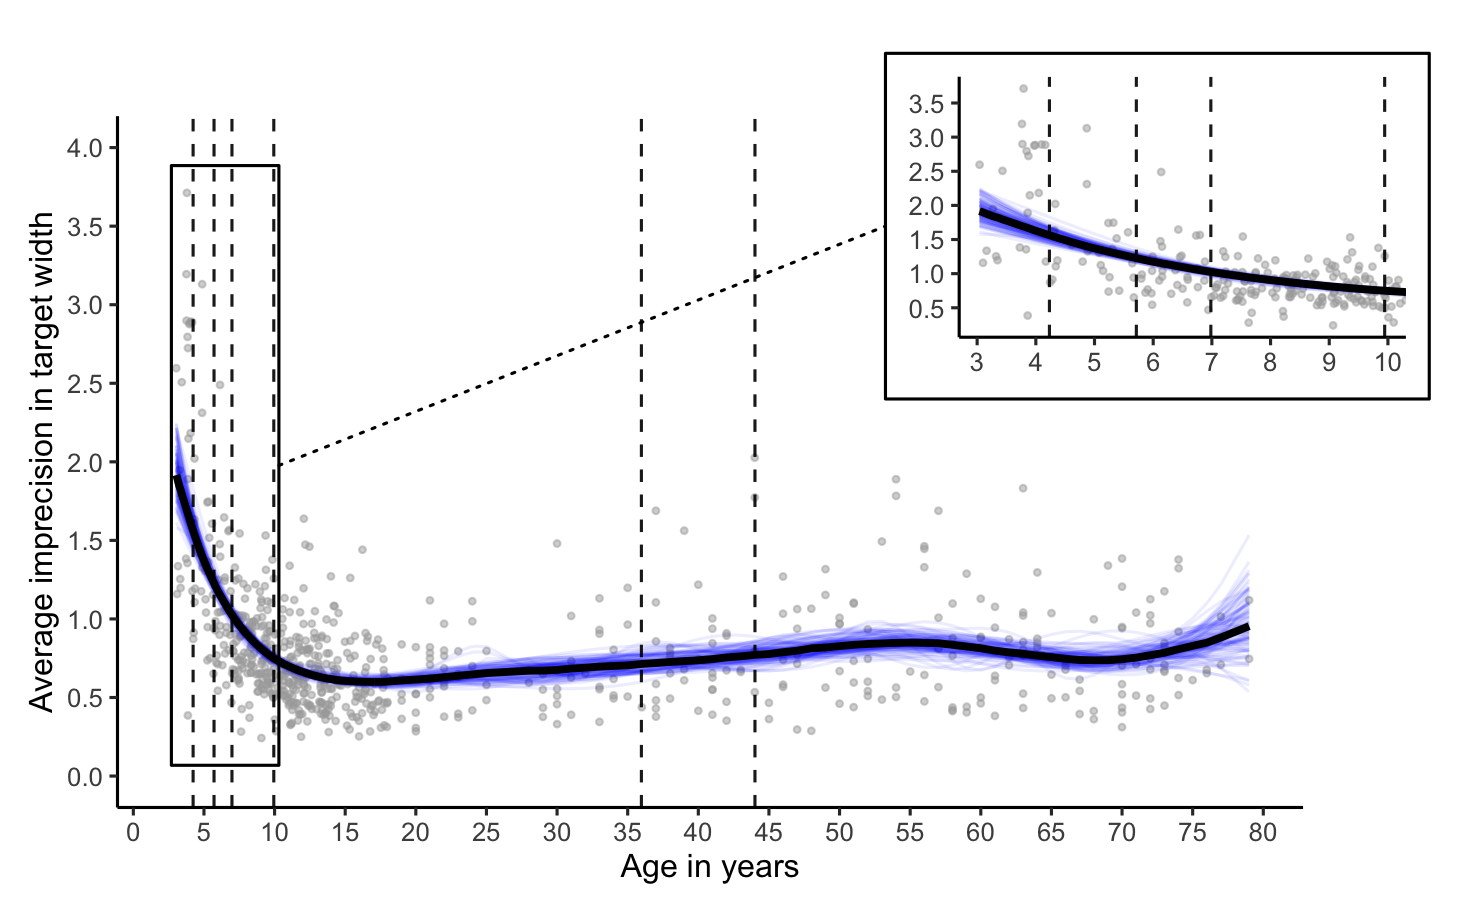
\includegraphics[width=1\linewidth]{../figures/lifespan_plot} 

}

\caption{\textbf{Developmental trajectory of gaze understanding across the lifespan}. Grey dots show the mean level of imprecision (ie., absolute distance between the target's center and the participant's click) for each subject averaged across trials. The unit of imprecision is counted in target width, i.e., a participant with imprecision of 1 clicked on average one target width to the left or right of the true target center. Blue lines show 100 draws from the expectation of the posterior predictive distribution of the Gaussian Process model, with its mean predicted developmental trajectory as a solid black line. Vertical, black, dashed lines show the locations of the most prominent changes according to our Bayesian change point analysis.}\label{fig:fig1}
\end{figure}

High levels of variation pointed to substantial individual differences in all age groups (overall imprecision mean = 0.81, sd = 0.82, range = {[}0 - 10.73{]}). We found substantial evidence for a non-linear development in gaze understanding across the lifespan. The Gaussian process model was clearly preferred over the polynomial models due to the highest predictive accuracy according to the LOO ELPD estimates: elpd\_diff between Gaussian process and cubic model = -33.75 (SE = 8.83); elpd\_diff between Gaussian process and quadratic model = -95.07 (SE = 15.19); elpd\_diff between Gaussian process and linear model = -127.17 (SE = 18.18); all in favor of the Gaussian process model. Moreover, the Gaussian Process model showed the greatest model weight (approximating 1). For the imprecision in gaze understanding, the standard deviation (\emph{b} = 1.52, 95\% CrI {[}0.25; 5.19{]}) indicated nonlinearity.

The Bayesian change point analysis revealed 6 major shifts in gaze understanding during the lifespan (MAP estimate with 23.49\% probability). The change points occurred at 4.23 (95\% CrI {[}4.13; 4.33{]}); 5.71 (95\% CrI {[}5.38; 5.90{]}); 6.98 (95\% CrI {[}6.64; 8.04{]}); 9.94 (95\% CrI {[}8.66; 12.55{]}); 35.97 (95\% CrI {[}27.30; 39.69{]}); and 44.01 years (95\% CrI {[}40.37; 44.43{]}). In short: we found a rapid initial improvement in gaze understanding in early childhood, followed by a long period of minor, very slow change with slightly increasing levels of imprecision toward old age.

\hypertarget{discussion}{%
\subsection{Discussion}\label{discussion}}

We investigated the shape of change in gaze understanding across the lifespan and found a non-linear developmental trajectory, in which young children quickly enhanced their level of proficiency. Performance peaked around early adulthood, while there was a minor decay in later adulthood. This is consistent with the view that humans fine-tune their existing gaze understanding ability after the first emergence in infancy. Furthermore, we observed substantial individual differences in all age groups. While variation was highest in the three- and four-year-olds, it remained relatively stable across the lifespan.

Previous studies found that children start to follow gaze in the second half of their first year of life (e.g., Moll \& Tomasello, 2004). In our sample, three-year-olds were still rather imprecise in their gaze understanding ability (average imprecision was approx. two target widths). How can we explain this divergence? First, we used subtle eye movements as cues. Many existing studies let the agents move eye and head in parallel (Behne et al., 2005; Povinelli et al., 1997), establishing a confound with the more salient head movement. Relying exclusively on eye movements might be more difficult for children than presenting them with a combined eye and head orientation (Carpenter et al., 1998). Silverstein et al. (2021) used a similar manipulation of gaze cues without head rotation and found that 6- to 18-month-olds were around or just above chance for gaze-following. The authors argue that infants might fixate on another's face most of the time, while eye movement alone might not be strong enough to guide their attention. Furthermore, our study required participants to (1) precisely follow an agent's gaze, (2) interpret this as a cue, and (3) use the cue to guide their own behavior. It is conceivable that three-year-olds followed the agent's gaze but did not translate this into precise, active behavior. Moll and Kadipasaoglu (2013) argue that social forms of perspective-taking evolve prior to visual perspective-taking, which only emerges within the third year of life. Young children might simply not be interested in a differential, spatial representation of the surrounding objects. Taken together, this might explain why our younger participants located the agent's gaze rather imprecisely.

Regarding our sample of elderly adults, we expect a sampling bias (Bethlehem, 2010; Gosling et al., 2004; Remillard et al., 2014). First, certainly not all older people have a high-speed internet connection or are knowledgeable in its use. Second, it takes motivation to participate in \emph{Prolific} studies. The elderly adults participating in \emph{Prolific} studies might show greater cognitive flexibility compared to their offline counterparts. Therefore, a representative sample may show a greater age decline in gaze understanding compared to our reported sample. In addition, older people might be more likely to suffer from visual impairments. Even though we filtered participants to only include normal- to correct-to-normal vision, we cannot guarantee that our participants showed no symptoms of reduced vision.

\hypertarget{study-2-computational-cognitive-model}{%
\section{Study 2: Computational cognitive model}\label{study-2-computational-cognitive-model}}

Our lifespan study showed that gaze understanding develops throughout childhood, and variation between individuals appears in all age groups. The TANGO has previously been shown to reliably capture inter-individual differences in gaze understanding (Prein et al., 2023). The variation between participants was thus likely genuine and not due to random noise. In Study 2, we aimed to understand the developmental change and individual differences on a process level. We present a theory of gaze understanding that explains how participants process the available gaze information to identify the agent's focus. We formalized this inference process in a computational cognitive model that replicates a schematic representation of how participants make inferences in the task's context (i.e., model of the task and not the data).

The study design and procedure obtained ethical clearance in the same way as Study 1 and was pre-registered: \url{https://osf.io/r3bhn}. Data were collected between May and August 2021.

\hypertarget{computational-model}{%
\subsection{Computational model}\label{computational-model}}

A formal definition of our computational cognitive model can be found in the Appendix. Broadly summarizing, our gaze model assumes participants to click at a certain point where two estimated gaze vectors meet. Each of these gaze vectors implies an estimated pupil angle for each eye that results from connecting the center of the agent's eyeball and the center of the pupil (see Figure \ref{fig:fig2}A). These angles are sampled from a product of two independent Normal distributions with equal variance, which are centered around the true pupil angles. Development of gaze understanding corresponds to a decrease in variance of the Normal distributions and, therefore, a more precise localization of the attentional focus of the agent.

The geometry of our model leads to a testable group-level prediction: the model predicted that TANGO trials vary in difficulty (see Figure \ref{fig:fig2}B and C): participants should be more imprecise in locating the target the further out it lands, resulting in a U-shaped pattern. If our data matched the pattern of this model prediction, this could act as evidence for the gaze model. Therefore, our gaze model provides a quantitative theory of gaze understanding. In the following, we tested these predictions in children and adults.



\begin{figure}

{\centering 
\includegraphics[width=1\linewidth]{../figures/gazemodel} 

}

\caption{\textbf{Gaze model} (A) Visualization of the gaze model (simplified, for one eye). Participants are assumed to observe the pupil location and estimate the center of the agent's eye. Connecting these two point estimates as a line yields the unique vector that extends from the center of the agent's eyeball through the center of the pupil to the attentional focal point. The angle between this vector and a line pointing vertically to the ground (black dashed line) is the pupil angle (\(\alpha\)). Participants are assumed to sample (grey lines) from Normal distributions (blue line) centered around the true pupil angle. The variance of the Normal distribution (\(\sigma_v\)) is expected to vary between participants. (B \& C) Geometrical features of the gaze model. As the pupil angle varies, a fixed amount of uncertainty in the angle corresponds to a varying degree of uncertainty in the estimated target location. The distribution around the target location from which participants sample is wider when the agent gazes toward the side than when she gazes centrally. The blue line on the ground shows the added level of uncertainty in the estimated target position for the target location further outward (C).}\label{fig:fig2}
\end{figure}

\hypertarget{participants-1}{%
\subsection{Participants}\label{participants-1}}

The sample consisted of 60 children, including 20 three-year-olds (mean age = 3.47 years, SD = 0.34, range = 3.07 - 3.97, 11 girls), 20 four-year-olds (mean age = 4.61 years, SD = 0.26, range = 4.09 - 4.98, 10 girls), 20 five-year-olds (mean age = 5.66 years, SD = 0.24, range = 5.01 - 5.96, 12 girls). Children were recruited via an internal database, where each parent previously consented to child development studies, and data was collected in kindergartens in Leipzig, Germany.

In addition, we included 50 adults from Study 1 (mean age = 31.92 years, SD = 12.15, range = 18 - 63, 36 female). Since developmental change was minimal in our adult sample (see Study 1) and the cognitive models were computationally heavy, we decided to only include the first 50 adults who had completed the study.

\hypertarget{procedure-1}{%
\subsection{Procedure}\label{procedure-1}}

We applied the same procedure as in Study 1. Children were tested in a quiet room in their kindergarten, while an experimenter guided the child through the study on a tablet. Adults participated online.

\hypertarget{analysis-1}{%
\subsection{Analysis}\label{analysis-1}}

We quantified how well our gaze model explained the gaze understanding process in two ways. First, we aggregated the model predictions and data for each target bin and age group (3-, 4-, 5-years-olds, adults), and computed correlation to quantify how well the model was able to recover the data. Second, we compared the predictions of our gaze model to two simple alternative models that assume participants do not rely on the agent's gaze at all: a random guessing model and a center bias model. The random guessing model assumed participants randomly clicked on the screen and was implemented as sampling from a uniform distribution over all possible coordinates, \(\mathcal{U}(0, 1920)\). The center bias model assumed participants always clicked near the screen center and was implemented as sampling from a Normal distribution with the screen center as the mean, and one balloon width as the variance, \(\mathcal{N}(960, 160)\). Note that the center bias model also predicted imprecision should be higher for targets further out on the screen. However, compared to the gaze model, it predicted a steep effect towards the sides, resulting in a V-shaped pattern (imprecision as the distance between the target location and the screen center). All cognitive models were implemented in WebPPL (Goodman \& Stuhlmüller, 2014).

We compared models via the marginal likelihood of the data under each model. The pairwise ratio of marginal likelihoods for two models is also known as the Bayes Factor, which quantifies the quality of a model's predictions by averaging over the possible values of the model's parameters weighted by the prior probabilities of those parameter values. It can be used to estimate how much more likely the data under one model are compared to the other. Bayes Factors implicitly consider model complexity: models with more parameters often have broader prior distributions over parameters, which might weaken potential gains in predictive accuracy.

\hypertarget{results-1}{%
\subsection{Results}\label{results-1}}

We found very clear support for our gaze model, both in children as well as adults. A strong correlation between the data mean and the gaze model estimate (\(\sigma_v\)) showed that the data mean is suitable to quantify individual differences: child sample \emph{r} = 0.95, 95\%CI {[}0.92, 0.97{]}; adult sample \emph{r} = 0.96, 95\%CI {[}0.93, 0.98{]}). The gaze model predicted a U-shaped pattern which we also observed in our data (see Figure \ref{fig:fig3}C). The model comparison strongly favored our gaze model over the center bias model (child sample \(logBF_{10}\) = 1,015.33; adult sample \(logBF_{10}\) = 2,575.75) and the random guessing model (child sample \(logBF_{10}\) = 388.98; adult sample \(logBF_{10}\) = 919.03). For the child sample, we went one step further into the analysis. When correlating the observed data across all target positions with the predictions of the three models, we found a high similarity for the gaze model: \emph{r} = 0.95, 95\%CI {[}0.90, 0.98{]}, while the correlations with the alternative models were smaller (center bias model: \emph{r} = 0.77, 95\%CI {[}0.57, 0.89{]}; random guessing model: \emph{r} = 0.78, 95\%CI {[}0.58, 0.89{]}). The gaze model's prior over potential target locations assumed that participants' clicks would be skewed towards the screen center. For children, we estimated the width of the prior's distribution based on the participants' age. Interestingly, we found that the differential age effects on the center bias prior were minor (intercept = 300.14, 95\%HDI {[}277.19; 321.28{]}; slope = 1.18, 95\%HDI {[}0.00; 18.78{]}). The slope of the prior indicated that older children were only marginally less drawn towards the screen center compared to the younger children.



\begin{figure}

{\centering 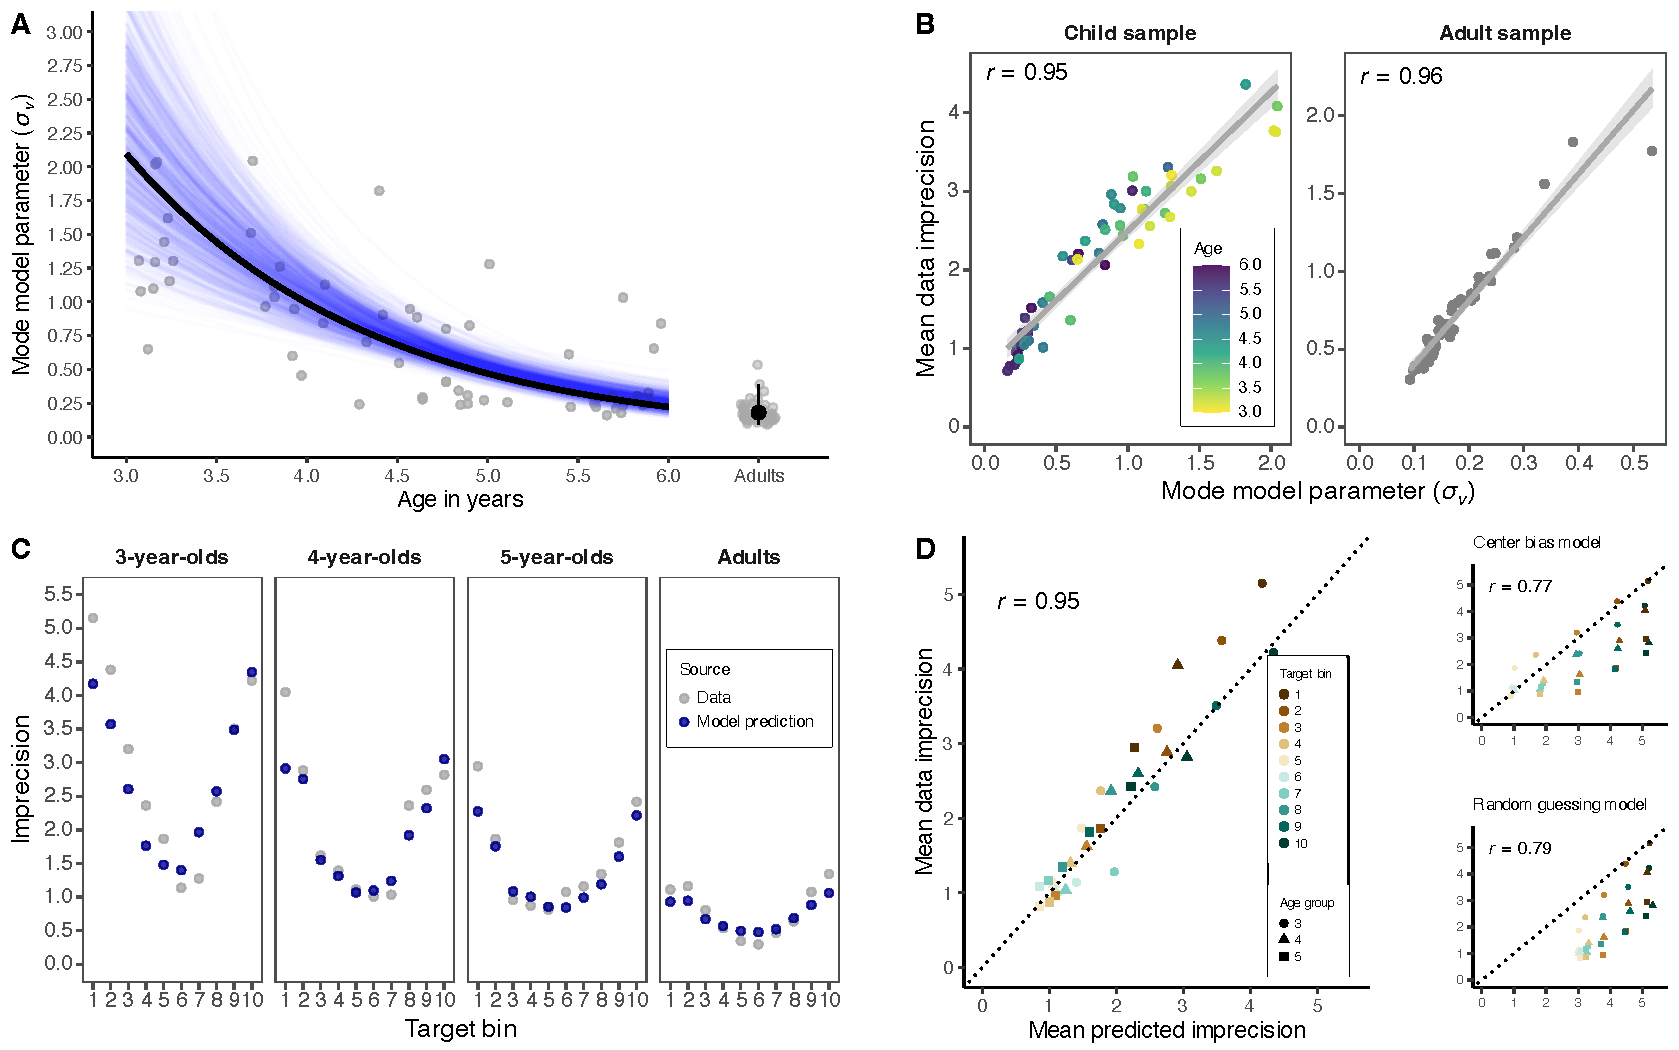
\includegraphics[width=1\linewidth]{../figures/gazemodel_plot} 

}

\caption{\textbf{Gaze model} (A) Developmental trajectory of the estimated model parameter. Grey dots show individual level parameter values. The black line shows the maximum a posteriori (MAP) estimate; blue lines show 1000 draws from it. The large black point with 95\% HDI shows the mean of the model parameter for the adult sample. We added minimal horizontal and vertical noise to the adult individual level parameter values to avoid overplotting. (B) Correlation between estimated mode of the model parameter and data mean per individual, faceted by age group. In the child sample, color denotes age in years. Grey regression lines with 95\% CI show smooth conditional means based on linear models, with \emph{Pearson}'s correlation coefficient \emph{r}. (C) Pattern recovery. Imprecision in target width for each target bin by age group. Model predictions in blue; data in grey. (D) Correlation between the observed data and the predictions of the three models by target position (across age and individuals; only for the child sample).}\label{fig:fig3}
\end{figure}

\hypertarget{discussion-1}{%
\subsection{Discussion}\label{discussion-1}}

We presented a formal cognitive model of gaze understanding to describe how gaze understanding develops with age and varies between individuals. We modeled gaze understanding as a process in which participants estimate pupil angles based on the pupil location within the eye. By following the resulting gaze vector, they consequently arrive at the attentional focus of the agent. Individual differences can be explained as varying levels of imprecision in the pupil angle estimation. We assume the basic process of gaze understanding to be the same across the lifespan, though individuals become increasingly precise with age. By conducting model comparisons, we ruled out simpler explanations of the data.

In addition, we observed differences in performance depending on gaze location: participant data showed that precision levels dropped as the agent's gaze moved further away from the center. Our gaze model predictions recovered this ``signature pattern'' in the data. Future research could use this signature in the data as evidence of whether diverse communities employ the same inferential mechanism to solve the task, speaking for a shared cognitive architecture.

Interestingly, the U-shaped pattern in the TANGO task can be conceptually compared to the result patterns of Michelon and Zacks (2006): in their Level 1 perspective-taking task, an increased distance between the agent and the target decreased performance (i.e., reaction times). Targets closer to the midline were more easily traced than ones further away from the agent. The authors concluded that visual acuity is generally higher for locations on the vertical than the diagonal axis (``oblique effect''; (Appelle, 1972; Heeley et al., 1997; Mikellidou et al., 2015)). Not only is the increased imprecision for TANGO trials in which the target lands further out consistent with this finding, but our gaze model poses a viable explanation for this effect.

A limitation of our model is that we cannot disentangle how much of the participants' uncertainty comes from a noisy estimate of the agent's attentional focus and how much is due to imprecise clicking (e.g., experiencing motor issues, adding random noise to the click). However, we believe imprecise clicking to be of minor concern, since the children in our sample seemed determined in where they clicked and to not have issues with aiming or motor control (see precision in training trials).

A critical feature of our model is that it assumes gaze understanding to rely on vector estimation: subjects are modeled to calculate pupil angles which serve as gaze vectors to point to the attentional focus point of an agent. Even though this vector estimation component is a geometrical calculation, one must first interpret the agent's eyes as a relevant social stimulus. Therefore, our model describes gaze understanding as a particular form of vector estimation in a social context.

\hypertarget{study-3-components-of-gaze-understanding}{%
\section{Study 3: Components of gaze understanding}\label{study-3-components-of-gaze-understanding}}

Study 3 examined the components of gaze understanding and whether it can be fully reduced to physical vector estimation. The positive link between TANGO and social-environmental factors like age of childcare entry (Prein et al., 2023) underline how gaze understanding is integral to social interaction. Therefore, we expected associations between gaze understanding and other measures of social-cognitive abilities.

First, we experimentally isolated the vector estimation component of the TANGO. We designed a new non-social vector estimation task that shared all crucial design features of the TANGO. Second, we assessed children's social-cognitive abilities by administering a Theory of Mind (TOM) task battery, comprising four tasks from the ToM scale by Wellman and Liu (Wellman \& Liu, 2004) and two additional perspective-taking tasks (Flavell, Flavell, et al., 1981; Flavell, Everett, et al., 1981). We reasoned that the TANGO shares task demands with the non-social vector estimation task while it shares its social context with the ToM tasks. As stated in our pre-registration, we further assessed whether the two perspective-taking tasks related to gaze understanding. Our reasoning was that similar underlying mechanisms might be needed to solve these tasks since they require participants to take into account another person's point of view.

Data collection was pre-registered (\url{https://osf.io/xsqkt}) and took place in Leipzig, Germany, between February and March 2023.

\hypertarget{participants-2}{%
\subsection{Participants}\label{participants-2}}

The sample consisted of 102 children (mean age = 4.54 years, SD = 0.31, range = 3.99 - 5.03, 54 girls). Information on individual socio-economic status was not formally recorded.

\hypertarget{procedure-2}{%
\subsection{Procedure}\label{procedure-2}}

Children were tested in a quiet room in their kindergarten. An experimenter guided the child through the study. For maximum control of extraneous participant variables, we employed a within-subjects study design. Participants performed the tasks in this order: (1) non-social vector estimation task, (2) ToM task battery, (3) TANGO. We decided on a fixed order to compare participants' performance straight-forwardly with each other. To increase engagement and decrease fatigue or fuzziness, we switched between tablet tasks and tasks with personal interaction. We presented the non-social vector estimation task before the TANGO so that participants would not be biased to interpret the stimuli as ``agent-like''.

\hypertarget{non-social-vector-estimation}{%
\subsubsection{Non-social vector estimation}\label{non-social-vector-estimation}}

Modeling the structure of the TANGO, we designed a non-social vector estimation task. This task was presented on a tablet and used the concept of magnetism. On the upper part of the screen, there was a tube with a circular window, containing a gearwheel. On the floor, there was a magnet. The magnet got switched on (with a cartoon-like sound), whereupon the gearwheel moved towards the magnet. The gearwheel moved so that its center aligned with the magnet center while staying inside the circular window. Participants were then asked to locate the magnet. Access to the magnet's true location was manipulated by a wooden wall: participants either had full, partial, or no visual access to the true magnet location. Compared to the TANGO, the circular window acted functionally similar to the agent's eyeball, while the gearwheel acted similar to the pupil. Participants were expected to estimate a vector from the center of the circular window to the gearwheel and extend this as a line toward the ground to locate the magnet. We deliberately decided against displaying an arrow: we aimed to keep the mechanistic functions of the TANGO and magnet stimuli as similar as possible. In both cases, the starting point of the vector needs to be estimated by the participant. With an arrow, we would have drastically reduced the level of uncertainty, since the arrow already displays all information (arrow tip as the ``gaze'' direction). Furthermore, we wanted to avoid referential or iconic stimuli.

Children received 19 trials with one full visual access trial, two partial visual access trials, and 16 test trials. The first trial of each type comprised a voice-over description of the presented events. We conducted our analysis with 15 test trials (excluding the voice-over trial). The outcome variable was imprecision, defined as the absolute distance between the magnet's x coordinate and the x coordinate of the participant's click. Magnet coordinates were randomized: The full width of the screen was divided into ten bins; each bin occurred equally often, while the same bin could occur in two consecutive trials; and exact coordinates within each bin were randomly generated.

\hypertarget{tom-task-battery}{%
\subsubsection{ToM task battery}\label{tom-task-battery}}

We administered four tasks from the Wellman and Liu (2004) ToM scale (see Supplements for further detail). We excluded three tasks: the Diverse Desires task to avoid ceiling effects; and both tasks involving emotions (Belief Emotion and Real-Apparent Emotion), as we aimed at assessing the ``cold, cognitive'' (vs.~``emotional'') aspects of social cognition. We added two perspective-taking level-2 tasks (Flavell, Flavell, et al., 1981; Flavell, Everett, et al., 1981) with the aim of increasing the variability we can capture between individuals, and since we hypothesized that perspective-taking would rely on similar mechanisms than gaze understanding, both relying on another's person egocentric frame of reference.

\hypertarget{gaze-understanding}{%
\subsubsection{Gaze understanding}\label{gaze-understanding}}

As in Study 1 and 2, we presented children with the TANGO (Prein et al., 2023). To accentuate the social aspect of the TANGO, we exchanged the animal agents (used in the previous two studies) with human faces, which were modeled after the local population in appearance (already created for another project on cross-cultural similarities in gaze understanding (\url{https://osf.io/tdsvc})). This further highlighted the contrast (i.e., social vs.~non-social context) to the physical vector estimation task.\footnote{In an exploratory analysis, we compared children's imprecision levels in the TANGO task with animal vs.~human agents. Based on a GLMM analysis, we conclude that there was no evidence of a stable effect of stimulus choice. See Supplements for further detail.}

\hypertarget{analysis-2}{%
\subsection{Analysis}\label{analysis-2}}

By design, the TANGO and the non-social vector estimation task involved vector estimation. Based on our computational model, we expected children's performance in both tasks to correlate with each other. For each task, we calculated the mean level of imprecision for each subject and correlated them using \emph{Pearson's} correlation coefficient.

For the ToM battery, we aggregated the score of all solved tasks. Regarding the relationship between the two vector estimation tasks and the ToM measures, we could imagine two possible scenarios: (A) If gaze understanding recruited a social-cognitive ability beyond geometric vector estimation, we expected that ToM measures would correlate more strongly with the gaze understanding task than with the non-social vector estimation task. (B) If gaze understanding relied purely on task-specific geometric processes, then the correlation between gaze understanding and ToM measures would be comparable to the correlation between non-social vector estimation and the ToM measures. For the association between the aggregate ToM scores and the gaze understanding / non-social vector estimation tasks, we used \emph{Spearman's} rank correlation coefficients.

We compared the correlation between gaze understanding and ToM measures and the correlation between non-social vector estimation and ToM measures by using the Williams' test from the function \texttt{cocor.dep.groups.overlap} (designed for two dependent overlapping correlations) from the package \texttt{cocor} (Diedenhofen \& Musch, 2015).

To estimate which components best explain the gaze understanding score, we conducted a model comparison with GLMMs predicting the mean imprecision in gaze understanding by age, imprecision in non-social vector estimation, the ToM aggregate score, or the aggregate of the two perspective-taking tasks (subset of ToM battery; example of model notation in \texttt{R:\ tango\_mean\ \textasciitilde{}\ age\_centered\ +\ magnet\_scaled\ +\ perspective\_scaled}). The outcome variable was modeled by a lognormal distribution. We wanted to assess whether the ToM aggregate score or the singled-out perspective-taking score added additional explanatory value when predicting the gaze understanding score. We hypothesized that perspective-taking seemed most closely theoretically related to gaze understanding as in both cases the participant was asked to judge another person's point of view.

\hypertarget{results-2}{%
\subsection{Results}\label{results-2}}

Gaze understanding substantially correlated with the non-social vector estimation task, \emph{r} = 0.38, 95\%CI {[}0.20, 0.53{]} (see Figure \ref{fig:fig4}B). Despite the designed overlap in task demands, the two vector estimation tasks were not redundant: only a part of the variance in gaze understanding could be explained by non-social vector estimation.

ToM abilities did not correlate with gaze understanding (\(\rho\) = -0.12, 95\%CI {[}-0.31, 0.07{]}) or non-social vector estimation (\(\rho\) = -0.12, 95\%CI {[}-0.30, 0.08{]}), and the correlations did not differ from each other, Williams' test \emph{t}(99) = 0, \emph{p} = 1.

Interestingly, gaze understanding and perspective-taking correlated with each other, \(\rho\) = -0.29, 95\%CI {[}-0.46, -0.10{]}. Please note that the negative correlation can be explained by the measure of imprecision in the TANGO (i.e., the more imprecise gaze understanding, the less perspective-taking). Non-social vector estimation and perspective-taking did not correlate, \(\rho\) = -0.09, 95\%CI {[}-0.28, 0.10{]}. However, according to the Williams' test, the two correlations did not differ significantly from each other, \emph{t}(99) = -1.86, \emph{p} = 0.07.

Our model comparison revealed that gaze understanding was best predicted by a model including non-social vector estimation (\(\beta\) = 0.14, 95\% CrI {[}0.06; 0.21{]}) and perspective-taking (\(\beta\) = -0.10; 95\% CrI {[}-0.17, -0.03{]}), even when controlling for age (\(\beta\) = -0.14, 95\% CrI {[}-0.38, 0.10{]}) (see Figure \ref{fig:fig4}C and Supplements for the model comparison).



\begin{figure}

{\centering 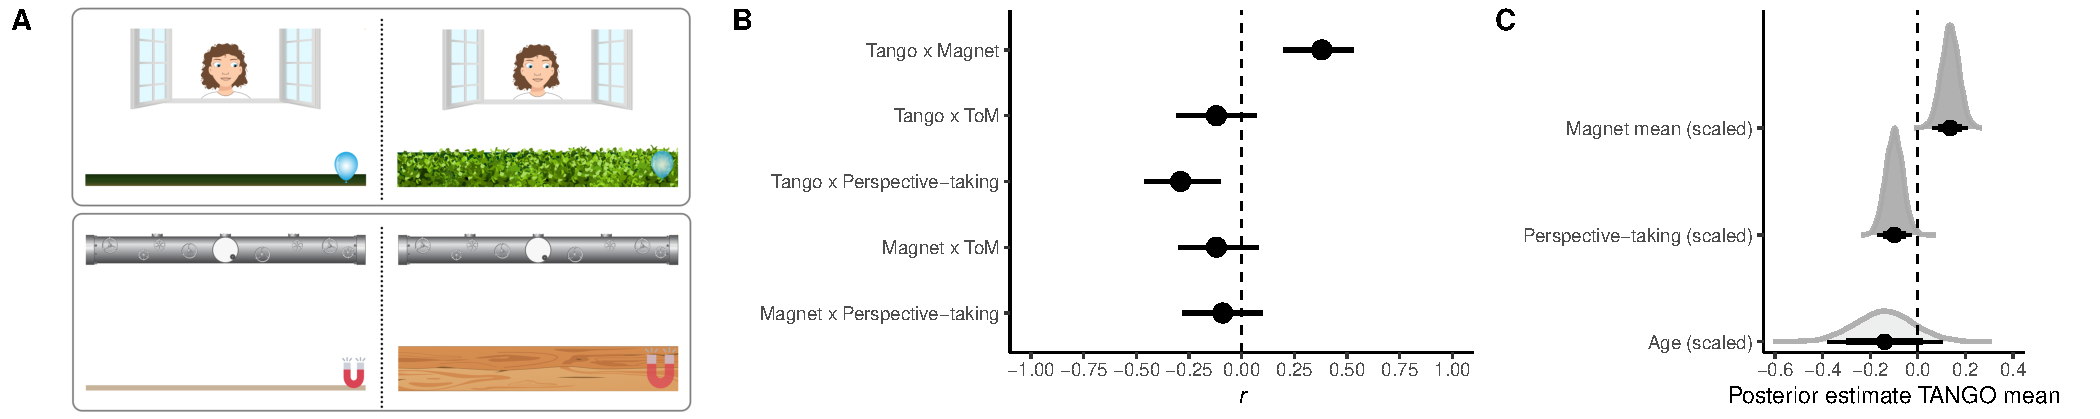
\includegraphics[width=1\linewidth]{../figures/magnet_plot} 

}

\caption{\textbf{Components of gaze understanding.} (A) Study procedures. Top: TANGO (i.e., gaze understanding; social vector estimation). Bottom: Magnet (i.e., non-social vector estimation). The left-hand side shows screenshots of the familiarization phase; right-hand side shows screenshots of the test phase. (B) Correlations between gaze understanding, physical vector estimation, ToM, and perspective-taking. Dots show the correlation coefficients, error bars represent 95\% CIs. (C) Influence of age, perspective-taking and physical vector estimation on gaze understanding. The graph shows the posterior distributions for the respective predictor. Black dots represent means, thicker black lines 80\% CrI, and thinner black lines 95\% CrI.}\label{fig:fig4}
\end{figure}

\hypertarget{discussion-2}{%
\subsection{Discussion}\label{discussion-2}}

Our gaze model assumed vector calculations on a process level. By isolating physical vector estimation experimentally, we could show that gaze understanding does indeed, to a certain degree, rely on this component. However, physical vector estimation alone did not suffice to explain variation in gaze understanding. Additionally, perspective-taking proved to be a relevant social-cognitive ability when predicting the performance in the TANGO (cf. Astor \& Gredebäck, 2022). The overall ToM aggregate score did not add explanatory power.

The TANGO and the two perspective-taking tasks can be seen as instances of visuospatial perspective-taking. Often, researchers distinguish between Level 1 and Level 2 perspective-taking tasks. Level 1 perspective-taking is concerned with the visibility of objects from a particular viewpoint (Surtees et al., 2013), and can usually be solved independently from another's agent frame of reference and without mental rotation {[}not matching the ``mentalizing criterion''; Quesque and Rossetti (2020){]}. In contrast, Level 2 perspective-taking tasks ask participants to judge how (visually or conceptually) the world looks for another person. Solving these tasks presumably relies on a simulation of mentally transforming one's own body schema into the space of another agent (Erle \& Topolinski, 2017). Participants must understand that different viewpoints lead to different perspectives (Flavell, Everett, et al., 1981): two agents can see the same object ``in different, incompatible, fine-grained ways'' (Rakoczy, 2022). In short, Level 1 perspective-taking addresses \emph{what} an agent can see, while Level 2 perspective-taking addresses \emph{how or where} they see it (Moll \& Tomasello, 2006). The TANGO falls into the first category - however, in contrast to existing research, on a continuous scale - while the perspective-taking tasks within our ToM scale fall into the second category.

In the TANGO, participants locate the target by assuming that another agent perceives and looks at the it. The here-applied Level 2 perspective-taking tasks add another layer by asking how one's perspective differs from another's and how exactly the other person sees an object. Michelon and Zacks (2006) assessed the different processes that participants used to master Level 1 and Level 2 perspective-taking tasks and concluded that participants rely on line-of-sight tracing in the former and perspective transformation in the latter case. Line-of-sight tracing consists of locating the avatar and the target, and drawing a line between them. Note how our gaze model in Study 2 shares the underlying idea of connecting points in space via a line. Level 2 perspective-taking requires an additional step in which participants ``perform a perspective transformation so that one's imagined position matches the position of the avatar'' (Michelon \& Zacks, 2006). Therefore, the processes to solve Level 1 perspective-taking tasks might be computationally lighter since there is no need to adapt the other person's reference frame. Still, the assumed processes overlap, which could explain the correlation between the TANGO and the administered perspective-taking tasks.

Surtees et al. (2013) further differentiated between visual and spatial perspective-taking. While the former helps to judge if and how an agent sees an object, the latter involves judging the relative spatial locations of an agent and the object. Spatial perspective-taking does not necessitate mental states since computing a line of sight does not demand the presence of another agent (Michelon \& Zacks, 2006) and can, therefore, be applied to non-agentive objects with a front (Surtees et al., 2013). This could explain how our participants solved the non-social vector estimation task.

Interestingly, we found weaker correlations between gaze understanding and the other ToM tasks. While the ToM tasks and the TANGO shared the social context, the cognitive processes needed to solve each task might vary. As Rakoczy (2022) reflected, perception-goal psychology (which includes gaze understanding) comprises understanding that others see different objects or pursue different goals. However, this ability does not necessarily entail understanding more complex meta-representational aspects; for example, understanding that mental states can be false or involve aspectual information.

In previous work, we established that the TANGO is suited to capture meaningful variability across individuals (Prein et al., 2023), which is a crucial task feature when we are interested in revealing the relationship between different cognitive abilities. Importantly, the tasks we used to measure ToM abilities were not designed to capture individual differences: the aggregate score of few dichotomous items is of limited use when it comes to quantifying genuine differences between individuals. However, since these tasks are the gold standard in the social-cognitive literature (Białecka-Pikul et al., 2021; Byom \& Mutlu, 2013; Poulin-Dubois et al., 2023; Rakoczy, 2022; Wellman, 2018), and measures with satisfying psychometric properties are, to the best of our knowledge, still scarce (e.g., Beaudoin et al., 2020; Mayes et al., 1996), we nonetheless relied on them in this study. Thus, lower correlations between ToM abilities and gaze understanding may reflect poor measurement characteristics on the side of ToM tasks rather than a genuine absence of association. We would like to point out that we already stated this concern in our pre-registration (\url{https://osf.io/xsqkt}).

If the reliability of the tasks at hand is known, one can estimate the ``true'' correlation between the latent constructs by applying an attenuation formula or structural equation models (Metsämuuronen, 2022; Trafimow, 2016). Adjusting for the measurement error would increase the so-called true correlation. While we can estimate the split-half reliability for the TANGO and the non-social vector estimation task (Prein et al., 2023), we do not have reliability estimates of the ToM measures and cannot apply said approaches. This, in turn, underlines the importance of reporting the psychometric properties of a task. The development of new measures to capture individual differences in social-cognitive abilities seems essential to move this research further.

\hypertarget{general-discussion}{%
\section{General discussion}\label{general-discussion}}

In three studies, we shed light on the cognitive process underlying gaze understanding and its developmental trajectory across the lifespan. Study 1 focused on how gaze understanding changes with age. We found a steep performance improvement in the preschool years in which children became more precise in locating the attentional focus of an agent. During teenage years and early adulthood, participants reached their peak performance. Precision levels then stayed comparably stable, with a minor decay toward older adulthood. Beyond these aggregated developmental patterns, we found that individual differences exist throughout the lifespan. In Study 2, we proposed a computational cognitive model that described gaze understanding at a process level. We modeled gaze understanding as a process in which participants use the pupil location within the eyes to estimate pupil angles. To locate the attentional focus of an agent (and find a target), they extend the resulting gaze vector towards the ground. Individuals vary in their levels of uncertainty around these pupil angles. Our gaze model outperformed two alternative models, which assumed participants solved the task via a center bias or random guessing. Knowing the TANGO to be a reliable individual differences measure, we investigated potential components of gaze understanding in Study 3. A fundamental assumption of our computational model was that gaze understanding relies on a vector estimation process. We experimentally isolated this component by designing a non-social vector estimation task. Furthermore, we assessed the relationship between gaze understanding and traditional ToM tasks. We found that gaze understanding does, indeed, share a substantial part of its variance with the non-social counterpart of physical vector estimation. Additionally, perspective-taking correlated with gaze understanding, whereas the other ToM measures (focussing on diverse desires, knowledge access, and false beliefs) did not.

The developmental trajectory seen in Study 1 shows how abilities that emerge in infancy can continue to develop throughout childhood. While previous research established that one-year-olds can orient their visual attention toward one out of two objects, this is not the end point of development. By studying gaze understanding on a continuum, we assessed not just \emph{whether}, but \emph{how precisely} children locate others' attentional focus. In previous work, we have shown that these individual differences are meaningful (e.g., connected to theoretically related constructs, and showing high split half and retest reliability; (Prein et al., 2023)). Capturing individual variation is crucial when we study development and the improvement in social-cognitive abilities.

Preschool children increased their precision level to locate an agent's attentional focus, which then stayed comparably stable across adulthood. Older adults decreased slightly in their precision levels. This developmental trajectory of a first emergence with a rapid improvement, followed by a plateau and slight decline toward older age, might be representative of many cognitive processes.

In Study 2, we proposed a theoretical framework to interpret the development and individual differences in gaze understanding. Our computational cognitive model assumes that participants estimate a pupil angle (i.e., the angle between a line extending vertically downwards from the pupil center and a line connecting the pupil and eye center; see Figure \ref{fig:fig2}A). The model parameter estimates a participant's latent ability to follow gaze and can explain why individuals differ in their precision to locate an agent's attentional focus. The model proposes that development in gaze understanding equals a reduction in noise when estimating the agent's pupil angles. We found strong evidence for the proposed gaze model when comparing it against two alternative models and correlating its predictions with the observed data (see Figure \ref{fig:fig3}D), both for children and adults. Notably, the model recovers signature patterns in the data (see Figure \ref{fig:fig3}C).

In Study 3, we tested the relation between gaze understanding and non-social vector estimation. As implied by our gaze model, we found that gaze understanding relates to the ability to estimate vectors in space. This ability might be helpful in several social-cognitive tasks, for example, action prediction (Friesen \& Rao, 2011), and intention understanding. Predicting which object another agent likely wants to grasp or calculating their movement pathway could rely on similar vector estimation abilities.

Even though our gaze model is designed within a 2D world, we believe the mechanisms can be extrapolated into the 3D world. The processes of understanding gaze in daily life likely rely on the same principles as proposed in this paper. We presented the first evidence that this might be the case. In Study 3, we administered Level 2 perspective-taking tasks in which participants needed to adapt another person's frame of reference in a real-world social interaction. The correlation between this task and the TANGO speaks toward a unified mechanism behind these two visual perspective-taking tasks, regardless of the testing setup (i.e., screen-based vs.~real-life interaction). Clearly, our real-life environment is visually more cluttered and diverse than the one presented in our tablet task. Here, however, additional informational sources are available to infer where others are looking; for example, body or head orientation or common ground (Bohn \& Köymen, 2018; Moll \& Kadipasaoglu, 2013; Osborne-Crowley, 2020). A previously shared interaction history might restrict the options we consider potential targets. From a modeling perspective, this might be represented as a non-uniform distribution over locations in the visual scenery.

While we described the development and mechanisms behind gaze understanding, we still need to further explore the driving forces behind this development. As seen in Prein et al. (2023), precision in gaze understanding is linked to receptive vocabulary and opportunities for social interaction (e.g., number of siblings and age when entering childcare). Humans likely learn to follow gaze in social interactions (Triesch et al., 2006). Which exact kind of interactions are most helpful to improve precision in gaze understanding remains unknown.

\hypertarget{limitations}{%
\section{Limitations}\label{limitations}}

In this paper, we have focused on studying variation across ages and individuals. However, our findings rely on participants from Western, Educated, Industrialized, Rich, and Democratic (WEIRD) backgrounds (Henrich et al., 2010). Cultural variation has been found in many foundational aspects of cognition and socialization: for example, in parent-child interaction and communicative signals (Nielsen et al., 2017). First evidence suggests that cultural variation in face-to-face interactions does not influence infants' gaze shifts (Hernik \& Broesch, 2019). While we cannot generalize our here-reported developmental trajectory to different socio-environmental settings, we predict that our presented process-model of gaze understanding holds true across communities. Analyzing cross-cultural variation and checking for predicted ``signature patterns'' in the data will inform our modeling work and theory building in further detail (Amir \& McAuliffe, 2020).

Moreover, our reported developmental trajectory in gaze understanding relied on a cross-sectional study. Longitudinal studies are needed to de-confound it from cohort effects and interpret the correlations between gaze understanding and other social-cognitive abilities.

We applied the same experimental paradigm for children, teenagers and adults alike. While this enables a direct comparison in performance across ages, it remains unclear whether the same method measures the same underlying psychological process in humans of different ages (Petersen, 2023). As we find strong evidence for our computational gaze model in children and adults, we are optimistic that our task is valid throughout the lifespan. Furthermore, the testing setup might have influenced different age groups differentially. Children and teenagers are likely more trained in using a tablet than the older adults in our sample. Recruiting older participants online might also select a particular subgroup of this age range. Seventy-year-olds who have working WIFI connections, know how to use a computer, and are registered on \emph{Prolific} might not be representative of their age group. We can imagine that results from a more diverse, in-person data collection might show different developmental trajectories toward old age.

Our computational model of gaze understanding estimates one person-specific parameter for how accurately participants locate another person's attentional focus. The model assumes no motor imprecision in this estimation. However, younger children could have located the agent's focus at one particular point but clicked somewhere slightly off for motor control reasons. This would blur the model's estimation of the inferential component. However, in the first training trial, in which children were simply asked to touch the balloon, we found nearly perfect precision levels (cf. Prein et al., 2023). Motor issues and inaccurate aiming, resulting in falsely wide estimations in the model's inferential component, seem unlikely.

In Study 3, we matched the non-social vector estimation task as closely as possible to the TANGO. However, a critical feature of the target object differed between the two tasks: in the TANGO, the target (= balloon) moved from the center of the screen to its final position in a self-propelled, continuous way. In the non-social vector estimation task, the target (= magnet) stayed stationary on the ground. Two possible critiques come to mind: first, the self-propelled movement of the balloon could evoke a sense of agency, which would not be the case for the magnet. Second, the starting positions differ: the magnet never appears in the center of the screen. Keeping the starting point of the balloon in mind might be especially important when interpreting the U-shaped pattern found in Study 2. Additionally, in the TANGO, two eyes are presented and information of the two (matching) cues needs to be integrated to infer the target's location. In the non-social vector estimation task, only one circular window with a gearwheel inside is presented as a directional cue, and there is no need to integrate two different information sources. Future research should investigate how factors like self-propelled movement, sense of agency, spatial layout, and number of information sources influence the mechanisms of gaze understanding.

\hypertarget{conclusion}{%
\section{Conclusion}\label{conclusion}}

In three studies, we have illuminated the development and the mechanisms of gaze understanding. We have shown that gaze understanding continues to develop beyond infancy, and that individuals differ in their precision levels to localize the attentional focus of an agent. Our proposed process-level theory successfully modeled the mechanisms of gaze understanding and the source of individual differences. The present research shows how precise and reliable measures and process models jointly inform each other and lead to a more comprehensive understanding of the psychological phenomenon in question.

\newpage

\hypertarget{references}{%
\section{References}\label{references}}

\begingroup
\setlength{\parindent}{-0.5in}
\setlength{\leftskip}{0.5in}

\hypertarget{refs}{}
\begin{CSLReferences}{1}{0}
\leavevmode\vadjust pre{\hypertarget{ref-amir2020crosscultural}{}}%
Amir, D., \& McAuliffe, K. (2020). Cross-cultural, developmental psychology: Integrating approaches and key insights. \emph{Evolution and Human Behavior}, \emph{41}(5), 430--444. \url{https://doi.org/10.1016/j.evolhumbehav.2020.06.006}

\leavevmode\vadjust pre{\hypertarget{ref-appelle1972perception}{}}%
Appelle, S. (1972). Perception and discrimination as a function of stimulus orientation: {The} "oblique effect" in man and animals. \emph{Psychological Bulletin}, \emph{78}(4), 266--278. \url{https://doi.org/10.1037/h0033117}

\leavevmode\vadjust pre{\hypertarget{ref-aslin2007look}{}}%
Aslin, R. N. (2007). What's in a look? \emph{Developmental Science}, \emph{10}(1), 48--53. \url{https://doi.org/10.1111/j.1467-7687.2007.00563.x}

\leavevmode\vadjust pre{\hypertarget{ref-astor2022gaze}{}}%
Astor, K., \& Gredebäck, G. (2022). Gaze following in infancy: {Five} big questions that the field should answer. In \emph{Advances in {Child Development} and {Behavior}} (p. S0065240722000192). Elsevier. \url{https://doi.org/10.1016/bs.acdb.2022.04.003}

\leavevmode\vadjust pre{\hypertarget{ref-astor2020social}{}}%
Astor, K., Lindskog, M., Forssman, L., Kenward, B., Fransson, M., Skalkidou, A., Tharner, A., Cassé, J., \& Gredebäck, G. (2020). Social and emotional contexts predict the development of gaze following in early infancy. \emph{Royal Society Open Science}, \emph{7}(9), 201178. \url{https://doi.org/10.1098/rsos.201178}

\leavevmode\vadjust pre{\hypertarget{ref-beaudoin2020systematic}{}}%
Beaudoin, C., Leblanc, É., Gagner, C., \& Beauchamp, M. H. (2020). Systematic {Review} and {Inventory} of {Theory} of {Mind Measures} for {Young Children}. \emph{Frontiers in Psychology}, \emph{10}, 2905. \url{https://doi.org/10.3389/fpsyg.2019.02905}

\leavevmode\vadjust pre{\hypertarget{ref-behne2005oneyearolds}{}}%
Behne, T., Carpenter, M., \& Tomasello, M. (2005). One-year-olds comprehend the communicative intentions behind gestures in a hiding game. \emph{Developmental Science}, \emph{8}(6), 492--499. \url{https://doi.org/10.1111/j.1467-7687.2005.00440.x}

\leavevmode\vadjust pre{\hypertarget{ref-bethlehem2010selection}{}}%
Bethlehem, J. (2010). Selection {Bias} in {Web Surveys}. \emph{International Statistical Review}, \emph{78}(2), 161--188. \url{https://doi.org/10.1111/j.1751-5823.2010.00112.x}

\leavevmode\vadjust pre{\hypertarget{ref-bialecka-pikul2021early}{}}%
Białecka-Pikul, M., Białek, A., Kosno, M., Stępień-Nycz, M., Blukacz, M., \& Zubek, J. (2021). Early mindreading scale: {From} joint attention to false-belief understanding. \emph{European Journal of Developmental Psychology}, \emph{0}(0), 1--18. \url{https://doi.org/10.1080/17405629.2021.1911799}

\leavevmode\vadjust pre{\hypertarget{ref-birch2017perspectives}{}}%
Birch, S. A. J., Li, V., Haddock, T., Ghrear, S. E., Brosseau-Liard, P., Baimel, A., \& Whyte, M. (2017). Perspectives on {Perspective Taking}. In \emph{Advances in {Child Development} and {Behavior}} (Vol. 52, pp. 185--226). Elsevier. \url{https://doi.org/10.1016/bs.acdb.2016.10.005}

\leavevmode\vadjust pre{\hypertarget{ref-bohn2019pervasive}{}}%
Bohn, M., \& Frank, M. C. (2019). The {Pervasive Role} of {Pragmatics} in {Early Language}. \emph{Annual Review of Developmental Psychology}, \emph{1}(1), 223--249. \url{https://doi.org/10.1146/annurev-devpsych-121318-085037}

\leavevmode\vadjust pre{\hypertarget{ref-bohn2018common}{}}%
Bohn, M., \& Köymen, B. (2018). Common {Ground} and {Development}. \emph{Child Development Perspectives}, \emph{12}(2), 104--108. \url{https://doi.org/10.1111/cdep.12269}

\leavevmode\vadjust pre{\hypertarget{ref-burkner2017brms}{}}%
Bürkner, P.-C. (2017). Brms: {An R Package} for {Bayesian Multilevel Models Using Stan}. \emph{Journal of Statistical Software}, \emph{80}(1), 1--28. \url{https://doi.org/10.18637/jss.v080.i01}

\leavevmode\vadjust pre{\hypertarget{ref-burkner2018advanced}{}}%
Bürkner, P.-C. (2018). Advanced {Bayesian Multilevel Modeling} with the {R Package} brms. \emph{The R Journal}, \emph{10}(1), 395. \url{https://doi.org/10.32614/RJ-2018-017}

\leavevmode\vadjust pre{\hypertarget{ref-butterworth1991minds}{}}%
Butterworth, G., \& Jarrett, N. (1991). What minds have in common is space: {Spatial} mechanisms serving joint visual attention in infancy. \emph{British Journal of Developmental Psychology}, \emph{9}(1), 55--72. \url{https://doi.org/10.1111/j.2044-835X.1991.tb00862.x}

\leavevmode\vadjust pre{\hypertarget{ref-byers-heinlein2021development}{}}%
Byers-Heinlein, K., Tsui, R. K.-Y., van Renswoude, D., Black, A. K., Barr, R., Brown, A., Colomer, M., Durrant, S., Gampe, A., Gonzalez-Gomez, N., Hay, J. F., Hernik, M., Jartó, M., Kovács, Á. M., Laoun-Rubenstein, A., Lew-Williams, C., Liszkowski, U., Liu, L., Noble, C., \ldots{} Singh, L. (2021). The development of gaze following in monolingual and bilingual infants: {A} multi-laboratory study. \emph{Infancy}, \emph{26}(1), 4--38. \url{https://doi.org/10.1111/infa.12360}

\leavevmode\vadjust pre{\hypertarget{ref-byom2013theory}{}}%
Byom, L., \& Mutlu, B. (2013). Theory of mind: Mechanisms, methods, and new directions. \emph{Frontiers in Human Neuroscience}, \emph{7}.

\leavevmode\vadjust pre{\hypertarget{ref-carpenter1998social}{}}%
Carpenter, M., Nagell, K., \& Tomasello, M. (1998). \href{https://www.ncbi.nlm.nih.gov/pubmed/9835078}{Social cognition, joint attention, and communicative competence from 9 to 15 months of age}. \emph{Monographs of the Society for Research in Child Development}, \emph{63}(4), i--vi, 1--143.

\leavevmode\vadjust pre{\hypertarget{ref-corkum1995development}{}}%
Corkum, V., \& Moore, C. (1995). Development of joint visual attention in infants. In \emph{Joint attention: {Its} origins and role in development} (pp. 61--83). Lawrence Erlbaum Associates, Inc.

\leavevmode\vadjust pre{\hypertarget{ref-corkum1998origins}{}}%
Corkum, V., \& Moore, C. (1998). The origins of joint visual attention in infants. \emph{Developmental Psychology}, \emph{34}(1), 28--38. \url{https://doi.org/10.1037/0012-1649.34.1.28}

\leavevmode\vadjust pre{\hypertarget{ref-dentremont1997demonstration}{}}%
D'Entremont, B., Hains, S. M. J., \& Muir, D. W. (1997). A demonstration of gaze following in 3- to 6-month-olds. \emph{Infant Behavior and Development}, \emph{20}(4), 569--572. \url{https://doi.org/10.1016/S0163-6383(97)90048-5}

\leavevmode\vadjust pre{\hypertarget{ref-deak2000effects}{}}%
Deák, G. O., Flom, R. A., \& Pick, A. D. (2000). \href{https://www.ncbi.nlm.nih.gov/pubmed/10902702}{Effects of gesture and target on 12- and 18-month-olds' joint visual attention to objects in front of or behind them}. \emph{Developmental Psychology}, \emph{36}(4), 511--523.

\leavevmode\vadjust pre{\hypertarget{ref-delbianco2019developmental}{}}%
Del Bianco, T., Falck-Ytter, T., Thorup, E., \& Gredebäck, G. (2019). The {Developmental Origins} of {Gaze-Following} in {Human Infants}. \emph{Infancy}, \emph{24}(3), 433--454. \url{https://doi.org/10.1111/infa.12276}

\leavevmode\vadjust pre{\hypertarget{ref-diedenhofen2015cocor}{}}%
Diedenhofen, B., \& Musch, J. (2015). Cocor: {A Comprehensive Solution} for the {Statistical Comparison} of {Correlations}. \emph{PLoS ONE}, \emph{10}(4), e0121945. \url{https://doi.org/10.1371/journal.pone.0121945}

\leavevmode\vadjust pre{\hypertarget{ref-emery2000eyes}{}}%
Emery, N. J. (2000). The eyes have it: The neuroethology, function and evolution of social gaze. \emph{Neuroscience \& Biobehavioral Reviews}, \emph{24}(6), 581--604. \url{https://doi.org/10.1016/S0149-7634(00)00025-7}

\leavevmode\vadjust pre{\hypertarget{ref-erle2017grounded}{}}%
Erle, T. M., \& Topolinski, S. (2017). The grounded nature of psychological perspective-taking. \emph{Journal of Personality and Social Psychology}, \emph{112}(5), 683--695. \url{https://doi.org/10.1037/pspa0000081}

\leavevmode\vadjust pre{\hypertarget{ref-flavell1981younga}{}}%
Flavell, J. H., Everett, B. A., Croft, K., \& Flavell, E. R. (1981). Young children's knowledge about visual perception: {Further} evidence for the {Level} 1--{Level} 2 distinction. \emph{Developmental Psychology}, \emph{17}, 99--103. \url{https://doi.org/10.1037/0012-1649.17.1.99}

\leavevmode\vadjust pre{\hypertarget{ref-flavell1981development}{}}%
Flavell, J. H., Flavell, E. R., Green, F. L., \& Wilcox, S. A. (1981). The {Development} of {Three Spatial Perspective-Taking Rules}. \emph{Child Development}, \emph{52}(1), 356--358. \url{https://doi.org/10.2307/1129250}

\leavevmode\vadjust pre{\hypertarget{ref-friesen2011gaze}{}}%
Friesen, A. L., \& Rao, R. P. N. (2011). Gaze {Following} as {Goal Inference}: {A Bayesian Model}. \emph{Proceedings of the Annual Meeting of the Cognitive Science Society}, \emph{33}(33).

\leavevmode\vadjust pre{\hypertarget{ref-frith2012mechanisms}{}}%
Frith, C. D., \& Frith, U. (2012). Mechanisms of {Social Cognition}. \emph{Annual Review of Psychology}, \emph{63}(1), 287--313. \url{https://doi.org/10.1146/annurev-psych-120710-100449}

\leavevmode\vadjust pre{\hypertarget{ref-gathercole2004structure}{}}%
Gathercole, S. E., Pickering, S. J., Ambridge, B., \& Wearing, H. (2004). The {Structure} of {Working Memory From} 4 to 15 {Years} of {Age}. \emph{Developmental Psychology}, \emph{40}, 177--190. \url{https://doi.org/10.1037/0012-1649.40.2.177}

\leavevmode\vadjust pre{\hypertarget{ref-goodman2014design}{}}%
Goodman, N. D., \& Stuhlmüller, A. (2014). \emph{The {Design} and {Implementation} of {Probabilistic Programming Languages}}.

\leavevmode\vadjust pre{\hypertarget{ref-gosling2004should}{}}%
Gosling, S. D., Vazire, S., Srivastava, S., \& John, O. P. (2004). Should {We Trust Web-Based Studies}? {A Comparative Analysis} of {Six Preconceptions About Internet Questionnaires}. \emph{American Psychologist}, \emph{59}(2), 93--104. \url{https://doi.org/10.1037/0003-066X.59.2.93}

\leavevmode\vadjust pre{\hypertarget{ref-gredeback2010development}{}}%
Gredebäck, G., Fikke, L., \& Melinder, A. (2010). The development of joint visual attention: A longitudinal study of gaze following during interactions with mothers and strangers. \emph{Developmental Science}, \emph{13}(6), 839--848. \url{https://doi.org/10.1111/j.1467-7687.2009.00945.x}

\leavevmode\vadjust pre{\hypertarget{ref-heeley1997oblique}{}}%
Heeley, D. W., Buchanan-Smith, H. M., Cromwell, J. A., \& Wright, J. S. (1997). The oblique effect in orientation acuity. \emph{Vision Research}, \emph{37}(2), 235--242. \url{https://doi.org/10.1016/S0042-6989(96)00097-1}

\leavevmode\vadjust pre{\hypertarget{ref-henrich2010weirdesta}{}}%
Henrich, J., Heine, S. J., \& Norenzayan, A. (2010). The weirdest people in the world? \emph{The Behavioral and Brain Sciences}, \emph{33}(2-3), 61-83; discussion 83-135. \url{https://doi.org/10.1017/S0140525X0999152X}

\leavevmode\vadjust pre{\hypertarget{ref-hernik2019infanta}{}}%
Hernik, M., \& Broesch, T. (2019). Infant gaze following depends on communicative signals: {An} eye-tracking study of 5- to 7-month-olds in {Vanuatu}. \emph{Developmental Science}, \emph{22}(4), e12779. \url{https://doi.org/10.1111/desc.12779}

\leavevmode\vadjust pre{\hypertarget{ref-hessels2020how}{}}%
Hessels, R. S. (2020). How does gaze to faces support face-to-face interaction? {A} review and perspective. \emph{Psychonomic Bulletin \& Review}, \emph{27}(5), 856--881. \url{https://doi.org/10.3758/s13423-020-01715-w}

\leavevmode\vadjust pre{\hypertarget{ref-ishikawa2022physiological}{}}%
Ishikawa, M., Senju, A., Kato, M., \& Itakura, S. (2022). Physiological arousal explains infant gaze following in various social contexts. \emph{Royal Society Open Science}, \emph{9}(8), 220592. \url{https://doi.org/10.1098/rsos.220592}

\leavevmode\vadjust pre{\hypertarget{ref-lempers1979young}{}}%
Lempers, J. D. (1979). Young {Children}'s {Production} and {Comprehension} of {Nonverbal Deictic Behaviors}. \emph{The Journal of Genetic Psychology}, \emph{135}(1), 93--102. \url{https://doi.org/10.1080/00221325.1979.10533420}

\leavevmode\vadjust pre{\hypertarget{ref-lempers1977development}{}}%
Lempers, J. D., Flavell, E. R., \& Flavell, J. H. (1977). \href{https://www.ncbi.nlm.nih.gov/pubmed/849832}{The development in very young children of tacit knowledge concerning visual perception}. \emph{Genetic Psychology Monographs}, \emph{95}(1), 3--53.

\leavevmode\vadjust pre{\hypertarget{ref-mayes1996testretest}{}}%
Mayes, L. C., Klin, A., Tercyak, K. P., Cicchetti, D. V., \& Cohen, D. J. (1996). Test-{Retest Reliability} for {False-Belief Tasks}. \emph{Journal of Child Psychology and Psychiatry}, \emph{37}(3), 313--319. \url{https://doi.org/10.1111/j.1469-7610.1996.tb01408.x}

\leavevmode\vadjust pre{\hypertarget{ref-meltzoff2010social}{}}%
Meltzoff, A. N., Brooks, R., Shon, A. P., \& Rao, R. P. N. (2010). {``{Social}''} robots are psychological agents for infants: {A} test of gaze following. \emph{Neural Networks}, \emph{23}(8), 966--972. \url{https://doi.org/10.1016/j.neunet.2010.09.005}

\leavevmode\vadjust pre{\hypertarget{ref-metsamuuronen2022attenuationcorrected}{}}%
Metsämuuronen, J. (2022). Attenuation-{Corrected Estimators} of {Reliability}. \emph{Applied Psychological Measurement}, \emph{46}(8), 720--737. \url{https://doi.org/10.1177/01466216221108131}

\leavevmode\vadjust pre{\hypertarget{ref-michel2021effects}{}}%
Michel, C., Kayhan, E., Pauen, S., \& Hoehl, S. (2021). Effects of {Reinforcement Learning} on {Gaze Following} of {Gaze} and {Head Direction} in {Early Infancy}: {An Interactive Eye-Tracking Study}. \emph{Child Development}, \emph{92}(4), e364--e382. \url{https://doi.org/10.1111/cdev.13497}

\leavevmode\vadjust pre{\hypertarget{ref-michelon2006two}{}}%
Michelon, P., \& Zacks, J. M. (2006). Two kinds of visual perspective taking. \emph{Perception \& Psychophysics}, \emph{68}(2), 327--337. \url{https://doi.org/10.3758/BF03193680}

\leavevmode\vadjust pre{\hypertarget{ref-mikellidou2015oblique}{}}%
Mikellidou, K., Cicchini, G. M., Thompson, P. G., \& Burr, D. C. (2015). The oblique effect is both allocentric and egocentric. \emph{Journal of Vision}, \emph{15}(8), 24. \url{https://doi.org/10.1167/15.8.24}

\leavevmode\vadjust pre{\hypertarget{ref-moll2013primacy}{}}%
Moll, H., \& Kadipasaoglu, D. (2013). The primacy of social over visual perspective-taking. \emph{Frontiers in Human Neuroscience}, \emph{7}.

\leavevmode\vadjust pre{\hypertarget{ref-moll200412}{}}%
Moll, H., \& Tomasello, M. (2004). 12- and 18-month-old infants follow gaze to spaces behind barriers. \emph{Developmental Science}, \emph{7}(1), F1--F9. \url{https://doi.org/10.1111/j.1467-7687.2004.00315.x}

\leavevmode\vadjust pre{\hypertarget{ref-moll2006level}{}}%
Moll, H., \& Tomasello, M. (2006). Level 1 perspective-taking at 24 months of age. \emph{British Journal of Developmental Psychology}, \emph{24}(3), 603--613. \url{https://doi.org/10.1348/026151005X55370}

\leavevmode\vadjust pre{\hypertarget{ref-moore2008development}{}}%
Moore, C. (2008). The {Development} of {Gaze Following}. \emph{Child Development Perspectives}, \emph{2}(2), 66--70. \url{https://doi.org/10.1111/j.1750-8606.2008.00052.x}

\leavevmode\vadjust pre{\hypertarget{ref-nielsen2017persistent}{}}%
Nielsen, M., Haun, D., Kärtner, J., \& Legare, C. H. (2017). The persistent sampling bias in developmental psychology: {A} call to action. \emph{Journal of Experimental Child Psychology}, \emph{162}, 31--38. \url{https://doi.org/10.1016/j.jecp.2017.04.017}

\leavevmode\vadjust pre{\hypertarget{ref-osborne-crowley2020social}{}}%
Osborne-Crowley, K. (2020). Social {Cognition} in the {Real World}: {Reconnecting} the {Study} of {Social Cognition With Social Reality}. \emph{Review of General Psychology}, \emph{24}(2), 144--158. \url{https://doi.org/10.1177/1089268020906483}

\leavevmode\vadjust pre{\hypertarget{ref-palan2018prolific}{}}%
Palan, S., \& Schitter, C. (2018). Prolific.ac---{A} subject pool for online experiments. \emph{Journal of Behavioral and Experimental Finance}, \emph{17}, 22--27. \url{https://doi.org/10.1016/j.jbef.2017.12.004}

\leavevmode\vadjust pre{\hypertarget{ref-perner2003perspective}{}}%
Perner, J., Brandl, J. L., Garnham, A., \& Peter Lang. (2003). What is a {Perspective Problem}? {Developmental Issues} in {Belief Ascription} and {Dual Identity}. \emph{Facta Philosophica}, \emph{5}(2), 355--378. \url{https://doi.org/10.5840/factaphil20035220}

\leavevmode\vadjust pre{\hypertarget{ref-petersen2023reexamining}{}}%
Petersen, I. T. (2023). \emph{Reexamining {Developmental Continuity} and {Discontinuity} in the 21st {Century}: {Better Aligning Behaviors}, {Functions}, and {Mechanisms}}. PsyArXiv. \url{https://doi.org/10.31234/osf.io/ghkm6}

\leavevmode\vadjust pre{\hypertarget{ref-pfeiffer2013gaze}{}}%
Pfeiffer, U. J., Vogeley, K., \& Schilbach, L. (2013). From gaze cueing to dual eye-tracking: {Novel} approaches to investigate the neural correlates of gaze in social interaction. \emph{Neuroscience \& Biobehavioral Reviews}, \emph{37}(10, Part 2), 2516--2528. \url{https://doi.org/10.1016/j.neubiorev.2013.07.017}

\leavevmode\vadjust pre{\hypertarget{ref-poulin-dubois2023discontinuity}{}}%
Poulin-Dubois, D., Goldman, E. J., Meltzer, A., \& Psaradellis, E. (2023). Discontinuity from implicit to explicit theory of mind from infancy to preschool age. \emph{Cognitive Development}, \emph{65}, 101273. \url{https://doi.org/10.1016/j.cogdev.2022.101273}

\leavevmode\vadjust pre{\hypertarget{ref-povinelli1997exploitation}{}}%
Povinelli, D. J., Reaux, J. E., Bierschwale, D. T., Allain, A. D., \& Simon, B. B. (1997). Exploitation of pointing as a referential gesture in young children, but not adolescent chimpanzees. \emph{Cognitive Development}, \emph{12}(4), 423--461. \url{https://doi.org/10.1016/S0885-2014(97)90017-4}

\leavevmode\vadjust pre{\hypertarget{ref-prein2023tango}{}}%
Prein, J. C., Kalinke, S., Haun, D. B. M., \& Bohn, M. (2023). {TANGO}: {A} reliable, open-source, browser-based task to assess individual differences in gaze understanding in 3 to 5-year-old children and adults. \emph{Behavior Research Methods}. \url{https://doi.org/10.3758/s13428-023-02159-5}

\leavevmode\vadjust pre{\hypertarget{ref-quesque2020theoryofmind}{}}%
Quesque, F., \& Rossetti, Y. (2020). What {Do Theory-of-Mind Tasks Actually Measure}? {Theory} and {Practice}. \emph{Perspectives on Psychological Science}, \emph{15}(2), 384--396. \url{https://doi.org/10.1177/1745691619896607}

\leavevmode\vadjust pre{\hypertarget{ref-rcoreteam2022language}{}}%
R Core Team. (2022). \emph{R: {A} language and environment for statistical computing} {[}Manual{]}. R Foundation for Statistical Computing.

\leavevmode\vadjust pre{\hypertarget{ref-rakoczy2022foundations}{}}%
Rakoczy, H. (2022). Foundations of theory of mind and its development in early childhood. \emph{Nature Reviews Psychology}, \emph{1}(4), 223--235. \url{https://doi.org/10.1038/s44159-022-00037-z}

\leavevmode\vadjust pre{\hypertarget{ref-remillard2014systematic}{}}%
Remillard, M. L., Mazor, K. M., Cutrona, S. L., Gurwitz, J. H., \& Tjia, J. (2014). Systematic {Review} of the {Use} of {Online Questionnaires} of {Older Adults}. \emph{Journal of the American Geriatrics Society}, \emph{62}(4), 696--705. \url{https://doi.org/10.1111/jgs.12747}

\leavevmode\vadjust pre{\hypertarget{ref-silverstein2021infants}{}}%
Silverstein, P., Feng, J., Westermann, G., Parise, E., \& Twomey, K. E. (2021). Infants {Learn} to {Follow Gaze} in {Stages}: {Evidence Confirming} a {Robotic Prediction}. \emph{Open Mind}, \emph{5}, 174--188. \url{https://doi.org/10.1162/opmi_a_00049}

\leavevmode\vadjust pre{\hypertarget{ref-surtees2013similarities}{}}%
Surtees, A., Apperly, I., \& Samson, D. (2013). Similarities and differences in visual and spatial perspective-taking processes. \emph{Cognition}, \emph{129}(2), 426--438. \url{https://doi.org/10.1016/j.cognition.2013.06.008}

\leavevmode\vadjust pre{\hypertarget{ref-tomasello2003makes}{}}%
Tomasello, M., \& Rakoczy, H. (2003). What {Makes Human Cognition Unique}? {From Individual} to {Shared} to {Collective Intentionality}. \emph{Mind and Language}, \emph{18}(2), 121--147. \url{https://doi.org/10.1111/1468-0017.00217}

\leavevmode\vadjust pre{\hypertarget{ref-trafimow2016attenuation}{}}%
Trafimow, D. (2016). The attenuation of correlation coefficients: A statistical literacy issue. \emph{Teaching Statistics}, \emph{38}(1), 25--28. \url{https://doi.org/10.1111/test.12087}

\leavevmode\vadjust pre{\hypertarget{ref-triesch2006gaze}{}}%
Triesch, J., Teuscher, C., Deák, G. O., \& Carlson, E. (2006). Gaze following: Why (not) learn it? \emph{Developmental Science}, \emph{9}(2), 125--147. \url{https://doi.org/10.1111/j.1467-7687.2006.00470.x}

\leavevmode\vadjust pre{\hypertarget{ref-vehtari2017practicala}{}}%
Vehtari, A., Gelman, A., \& Gabry, J. (2017). Practical {Bayesian} model evaluation using leave-one-out cross-validation and {WAIC}. \emph{Statistics and Computing}, \emph{27}(5), 1413--1432. \url{https://doi.org/10.1007/s11222-016-9696-4}

\leavevmode\vadjust pre{\hypertarget{ref-wellman2018theory}{}}%
Wellman, H. M. (2018). Theory of mind: {The} state of the art. \emph{European Journal of Developmental Psychology}, \emph{15}(6), 728--755. \url{https://doi.org/10.1080/17405629.2018.1435413}

\leavevmode\vadjust pre{\hypertarget{ref-wellman2004scaling}{}}%
Wellman, H. M., \& Liu, D. (2004). Scaling of {Theory-of-Mind Tasks}. \emph{Child Development}, \emph{75}(2), 523--541. \url{https://doi.org/10.1111/j.1467-8624.2004.00691.x}

\leavevmode\vadjust pre{\hypertarget{ref-zhao2019detecting}{}}%
Zhao, K., Wulder, M. A., Hu, T., Bright, R., Wu, Q., Qin, H., Li, Y., Toman, E., Mallick, B., Zhang, X., \& Brown, M. (2019). Detecting change-point, trend, and seasonality in satellite time series data to track abrupt changes and nonlinear dynamics: {A Bayesian} ensemble algorithm. \emph{Remote Sensing of Environment}, \emph{232}, 111181. \url{https://doi.org/10.1016/j.rse.2019.04.034}

\leavevmode\vadjust pre{\hypertarget{ref-zohary2022gaze}{}}%
Zohary, E., Harari, D., Ullman, S., Ben-Zion, I., Doron, R., Attias, S., Porat, Y., Sklar, A. Y., \& Mckyton, A. (2022). Gaze following requires early visual experience. \emph{Proceedings of the National Academy of Sciences}, \emph{119}(20), e2117184119. \url{https://doi.org/10.1073/pnas.2117184119}

\end{CSLReferences}

\endgroup

\newpage

\hypertarget{appendix}{%
\section{Appendix}\label{appendix}}

Our computational model in Study 2 quantified a participant's cognitive ability to follow gaze by inverting a probabilistic process that generates the participant's clicks from observing the eyes of the agent. It is formally defined as:

\begin{equation}
    P(\theta | x_c, \alpha_l, \alpha_r) \propto P(x_c | \alpha_l, \alpha_r, \theta)P(\theta)
\end{equation}

where \(\theta\) is an individual's cognitive ability to locate the focus of the agent's attention, \(x_c\) is the coordinate the participant clicked, and \(\alpha_l\) and \(\alpha_r\) are the pupil angles for the left and right eye, respectively. The pupil angle \(\alpha\) is defined as the angle between a line connecting the center of the eye to the pupil and a line extended vertically downward from the center of the eye (see Figure \ref{fig:fig2}A).

This model mirrors the logic of the TANGO programming code. In the online experiment, we read out the center point coordinates of the target and the agent's eyeball (i.e., the SVG coordinates), and then calculated a line between these two points: this was our gaze vector (acting in the functionally same way as a pupil angle). Knowing the eyeball radius, we calculated the point of intersection at which the gaze vector met the eyeball boundary. Finally, the agent's pupil moved from the center of the eyeball along the gaze vector to the intersection point. This way, the agent was animated to ``look at'' the target. In the gaze model, we assumed participants go through these steps in reverse order.

Based on our verbal task instructions, we assumed that participants (1) expected the agent's looks to be directed at the target, and (2) to click on the coordinate they estimated the agent to look at. Consequently, we did not assume that participants' clicks were noisy in any way but that they clicked on the screen location where they genuinely thought the target was (and that the agent was looking at).

The true eye angles (\(\alpha_l\) and \(\alpha_r\)) cannot be directly observed and have to be estimated based on the position of the pupils within the eyes, resulting in approximate values (\(\hat{\alpha_l}\) and \(\hat{\alpha_r}\)). We presumed this estimation to be a noisy process. Thus, we conceptualized the development of the cognitive ability to follow gaze as a reduction of noise in the estimates (i.e., an increased certainty about the pupil angles).

Any clicked value of \(x_c\) implied a ``matched pair'' of the estimated pupil angles \(\hat{\alpha_l}\) and \(\hat{\alpha_r}\), with the property that lines extended along those two angles met at the precise location of the target. As a consequence, we can rewrite the likelihood function of the model above:

\begin{equation}
P(x_c | \alpha_l, \alpha_r, \theta) \propto P(\hat{\alpha_l}, \hat{\alpha_r} | \alpha_l, \alpha_r, \theta) P(x_c)
\end{equation}

\(P(x_c)\) is a prior over potential target locations, which we assumed to be skewed towards the screen center: We anticipated that participants have an a priori expectation that the target will land close to the middle, because the target was last visible in the screen center before disappearing behind the hedge and because the agent was located centrally on the screen. We estimated the strength of this center bias (i.e., the standard deviation of a Normal distribution around the screen center) based on the data: \(P(x_c) \sim \mathcal{N}(960, \sigma^p)\).

The width of this distribution is defined by \(\sigma^p\). For children, we assumed that the center bias changed with age and estimated \(\sigma^p\) via a linear regression as a function of the child's age (\(age_i\)): \(\sigma^p = \beta_0^{\sigma^p} + age_i \cdot \beta_1^{\sigma^p}\). Therefore, the participant-specific distribution for \(P(x_c)\) was constrained by the performance in the TANGO and the child's age. For the adults, \(\sigma^p\) was not age-specific.

The main inferential task for the participant lay in estimating the pupil angles, i.e., sampling from the first term of the right-hand side equation above, \(P(\hat{\alpha_l}, \hat{\alpha_r} | \alpha_l, \alpha_r, \theta)\). For this, we assumed that the pair of estimated pupil angles were sampled from a probability distribution which is the product of two Normal distributions of equal variance, \(\sigma_v\), centered on the true pupil angles:

\begin{equation}
P(\hat{\alpha_l}, \hat{\alpha_r} | \alpha_l, \alpha_r, \theta) \propto \phi(\hat{\alpha}_l ; \alpha_l, \sigma_v)\phi(\hat{\alpha}_r ; \alpha_r, \sigma_v),
\end{equation}

As \(\sigma_v\) determined the level of accuracy with which participants estimated the pupil angles, it is the component of the model that defines \(\theta\). When \(\sigma_v\) is very small (i.e., the distribution around the pupil angle is narrow), clicks far away from the target are unlikely, as these would require estimated pupil angles very different from the true pupil angles.~When \(\sigma_v\) is very large (i.e., the distribution around the pupil angle is wide), almost any pupil angles may be sampled, corresponding to a roughly uniform distribution over click coordinates. We expected \(\sigma_v\) to vary between individuals. Consequently, individuals differed in the level of precision with which they can locate the target based on observing the agent's eyes.

The shape of the \(P(x_c | \alpha_l, \alpha_r, \theta)\) distribution leads to a testable group-level prediction. As the pupil location varies, a fixed amount of uncertainty around the pupil angle corresponds to a varying degree of uncertainty in the estimated target location (see Figure \ref{fig:fig2}B \& C). When the agent directs their gaze toward the very left or right side, the distribution around the target location from which participants sample is comparatively wider than when the agent gazes centrally to the ground. For illustrative purposes, imagine a similar phenomenon: pointing a torch light to a flat surface on the ground. When one points the light cone directly at the surface, the light beam is concentrated in a clearly defined, small, symmetric area. When one points the light cone further away from oneself (shining at an angle), the light from one half of the cone must travel further to reach the surface than the light from the other half, resulting in an asymmetric light pattern. As the angle increases, the light is spread over a wider area, and the surface is illuminated less evenly. Consequently, for the same \(\sigma_v\), the further out a target coordinate lies, the wider and less symmetric the distribution. This increases both the variance and the bias in a participant's estimate of the agent's attentional focus, resulting in a decreased performance in the task. As \(\sigma_v\) decreases and the cone narrows, the extent to which performance varies at different angles decreases.

In our screen-based study, this effect should decrease again towards the most outward sides. Since the computer screen has a natural border, trials in which the target lands furthest out to the left/right become slightly easier again. In these cases, the uncertainty about the pupil angle faces practically only the inner side (facing the center) of the screen, since the natural border of the screen limits where participants can click. In another adult sample with more trials, we could recover this pattern. For further elaboration, see Supplements.


\end{document}
